\documentclass[a4paper,12pt]{report}

\usepackage[romanian]{babel}
\usepackage[a4paper,top=2cm,bottom=2cm,left=3cm,right=3cm,marginparwidth=1.75cm]{geometry}
\usepackage[colorlinks=true, allcolors=black]{hyperref}
\usepackage[nottoc,numbib]{tocbibind}
\usepackage{amsmath}
\usepackage{graphicx}
\usepackage{indentfirst}
\usepackage{enumitem}
\usepackage{placeins}
\usepackage{fontspec}
\usepackage{longtable}
\usepackage{array}

\setlength{\parindent}{5mm}
\setlength{\parskip}{6pt}

\setmainfont{UTSans}[
    Path=./fonts/,
    Extension = .ttf,
    UprightFont=*-Regular,
    BoldFont=*-Bold,
    ItalicFont=*-Regular,
    ItalicFeatures={FakeSlant=0.25}
]

\begin{document}
\section*{Scopul aplicației}
Aplicația are scopul de a facilita și automatiza gestionarea accesului în parcările auto, prin identificarea și înregistrarea automată a numerelor de înmatriculare ale autovehiculelor, aducând beneficii eficienței operaționale și securității.

\begin{figure}[h]
    \centering
    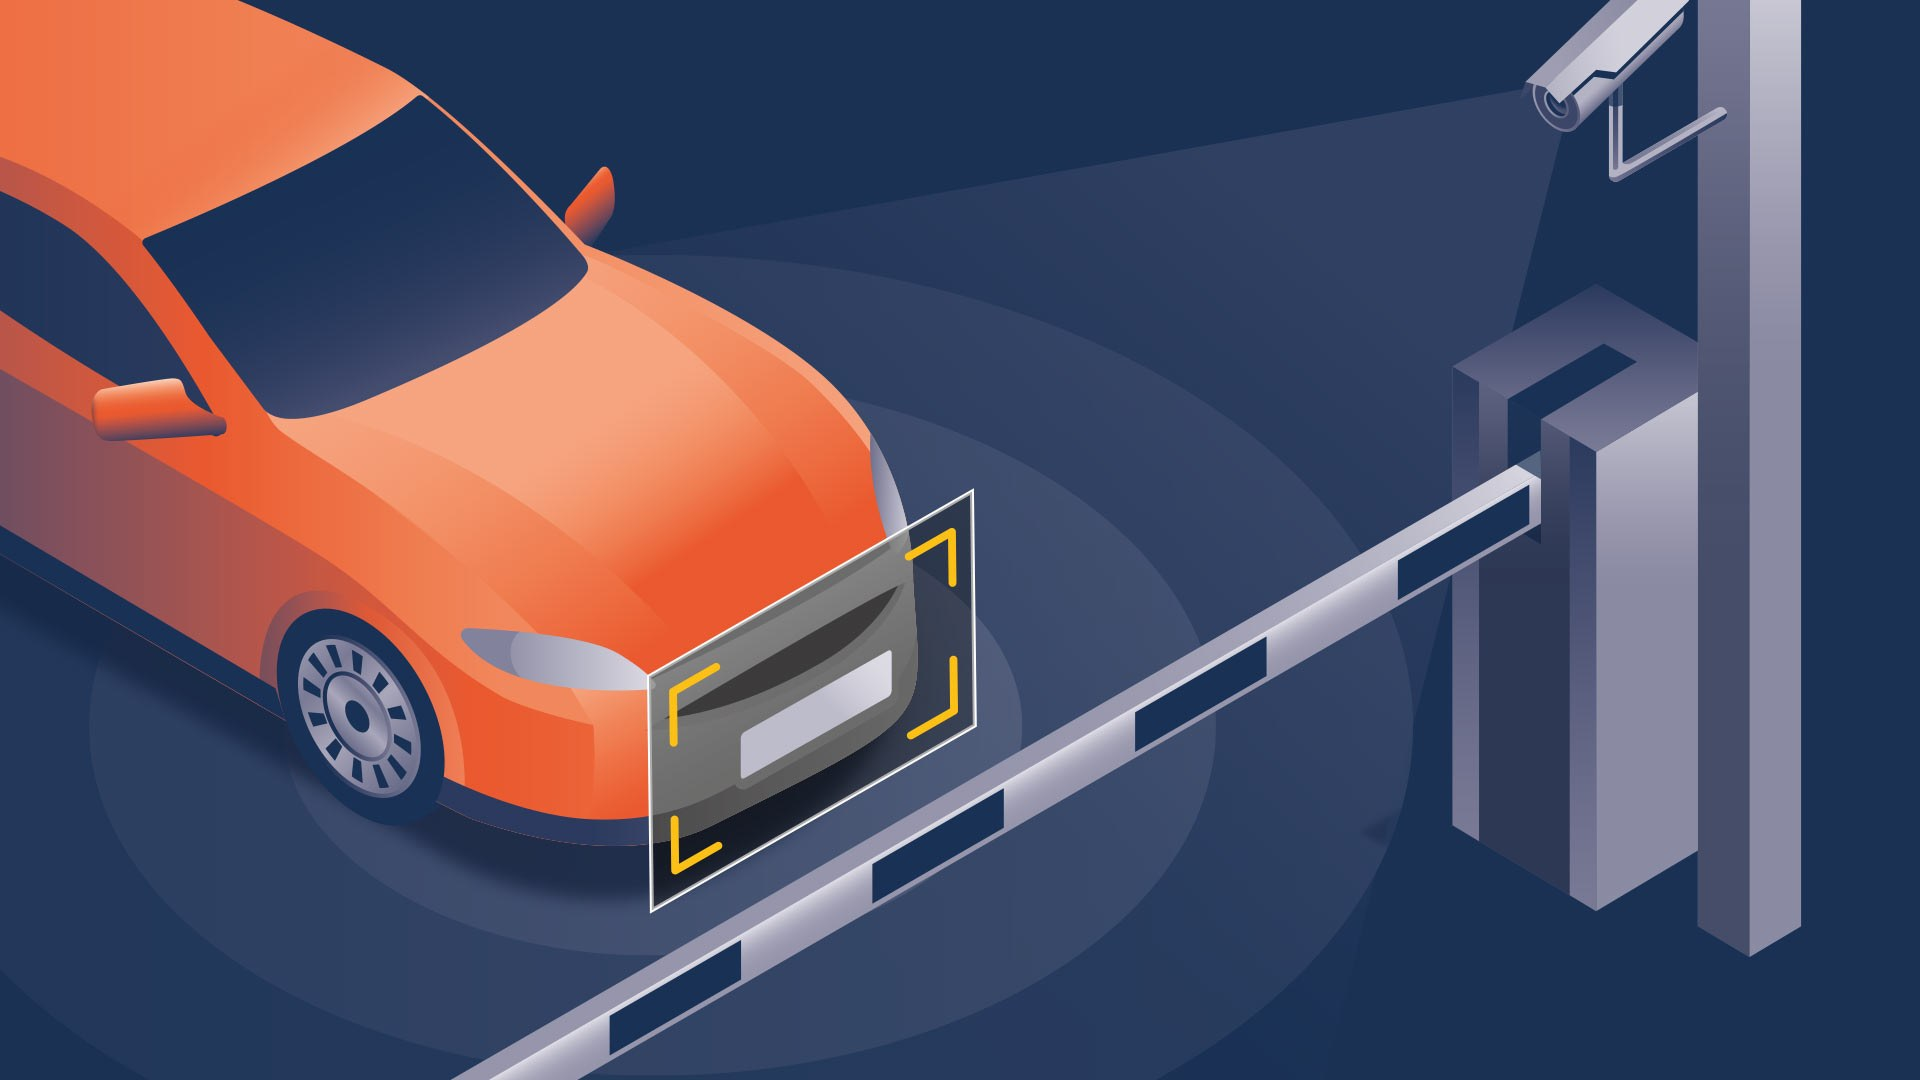
\includegraphics[width=0.7\textwidth]{images/picture.jpg}
\end{figure}
\FloatBarrier

\begin{enumerate}[label=\Roman*.]
    \item \textbf{Detectarea și identificarea automată a numărului de înmatriculare:} Aplicația utilizează camere video poziționate strategic pentru a capta imagini ale vehiculelor la momentul intrării sau ieșirii acestora din parcare. Aceste imagini sunt analizate în timp real pentru a se detecta și recunoaște numerele de înmatriculare.

    \item \textbf{Prelucrarea imaginilor:} Folosind algoritmi de procesare a imaginilor și tehnici de segmentare, aplicația extrage și rectifică numărul de înmatriculare din imaginea captată, asigurându-se că textul este clar în imagine.

    \item \textbf{Recunoașterea textului prin tehnologii de inteligență artificială:} Odată ce numărul de înmatriculare este izolat și optimizat, modelul AI Tesseract de recunoaștere optică a caracterelor (OCR) interpretează textul. Acest model este antrenat să recunoască în special fonturile și stilurile numerelor de înmatriculare.

    \item \textbf{Înregistrarea și monitorizarea accesului:} Numerele de înmatriculare recunoscute sunt înregistrate într-o bază de date. Aceasta permite urmărirea vehiculelor care intră și ies din parcare, oferind date importante pentru securitate și gestionarea spațiului de parcare.

    \item \textbf{Interfața grafică de utilizator (GUI):} Aplicația include o interfață grafică prietenoasă și intuitivă, care afișează în timp real informațiile despre accesul în parcare. Interfața permite utilizatorilor să vizualizeze imagini recente și să acceseze istoricul vehiculelor care au pătruns în parcare.
\end{enumerate}

\section*{Motivarea aplicației}
În cadrul proiectului, s-a urmărit dezvoltarea unei soluții eficiente prin valorificarea cunoștințelor existente din domeniul procesării imaginilor. Totodata, proiectul a implicat aplicarea și extinderea tehnicilor de analiză și procesare vizuală, pentru a identifica și extrage numerele de înmatriculare din imaginile captate de la intrările în parcările auto.

Ca limbaj de programare s-a optat pentru C++, care este larg recunoscut în domeniul procesării de imagini datorită eficienței sale remarcabile și a flexibilității pe care o oferă în gestionarea resurselor de sistem, contribuind la optimizarea timpului de execuție si permițând manipularea avansată și rapidă a datelor vizuale.

Pe parcursul dezvoltării soluției, s-a pus accent pe integrarea unei suite de tehnologii și instrumente de dezvoltare pentru a optimiza atât procesul de elaborare, cât și performanța finală a sistemului. În acest sens, s-a utilizat biblioteca OpenCV, care a fost esențială în lucrul cu imagini si utilizarea algoritmilor de procesare. De asemenea, s-a folosit modelul de inteligență artificială Tesseract OCR, recunoscut pentru eficiența sa în recunoașterea optică a caracterelor, pentru a extrage textul clar și precis din imagini.

Interfața grafică a fost creată cu ajutorul framework-ului Qt, oferind o manieră eficientă de interacțiune și o vizualizare intuitivă a datelor procesate. Pentru managementul proiectului și automatizarea construcției sistemului, s-au folosit CMake și Doxygen, acesta din urmă facilitând generarea documentației tehnice detaliate. De asemenea, pentru a asigura robustețea codului, s-au implementat unit teste, care au permis verificarea și validarea funcționalităților în diverse scenarii de utilizare.

Întregul proces de dezvoltare a fost suportat de mediul integrat de dezvoltare Visual Studio, și a fost gestionat folosind GitLab pentru versionarea codului.

\section*{Segmentarea, rectificarea și recunoașterea textului}
În continuare, dorim să aprofundăm pașii de execuție ai programului. În paralel, vom lua în considerare și o imagine drept exemplu pentru a ilustra fiecare etapă, oferind o perspectivă mai clară și mai cuprinzătoare asupra procesului de funcționare a aplicației.

\begin{figure}[h]
    \centering
    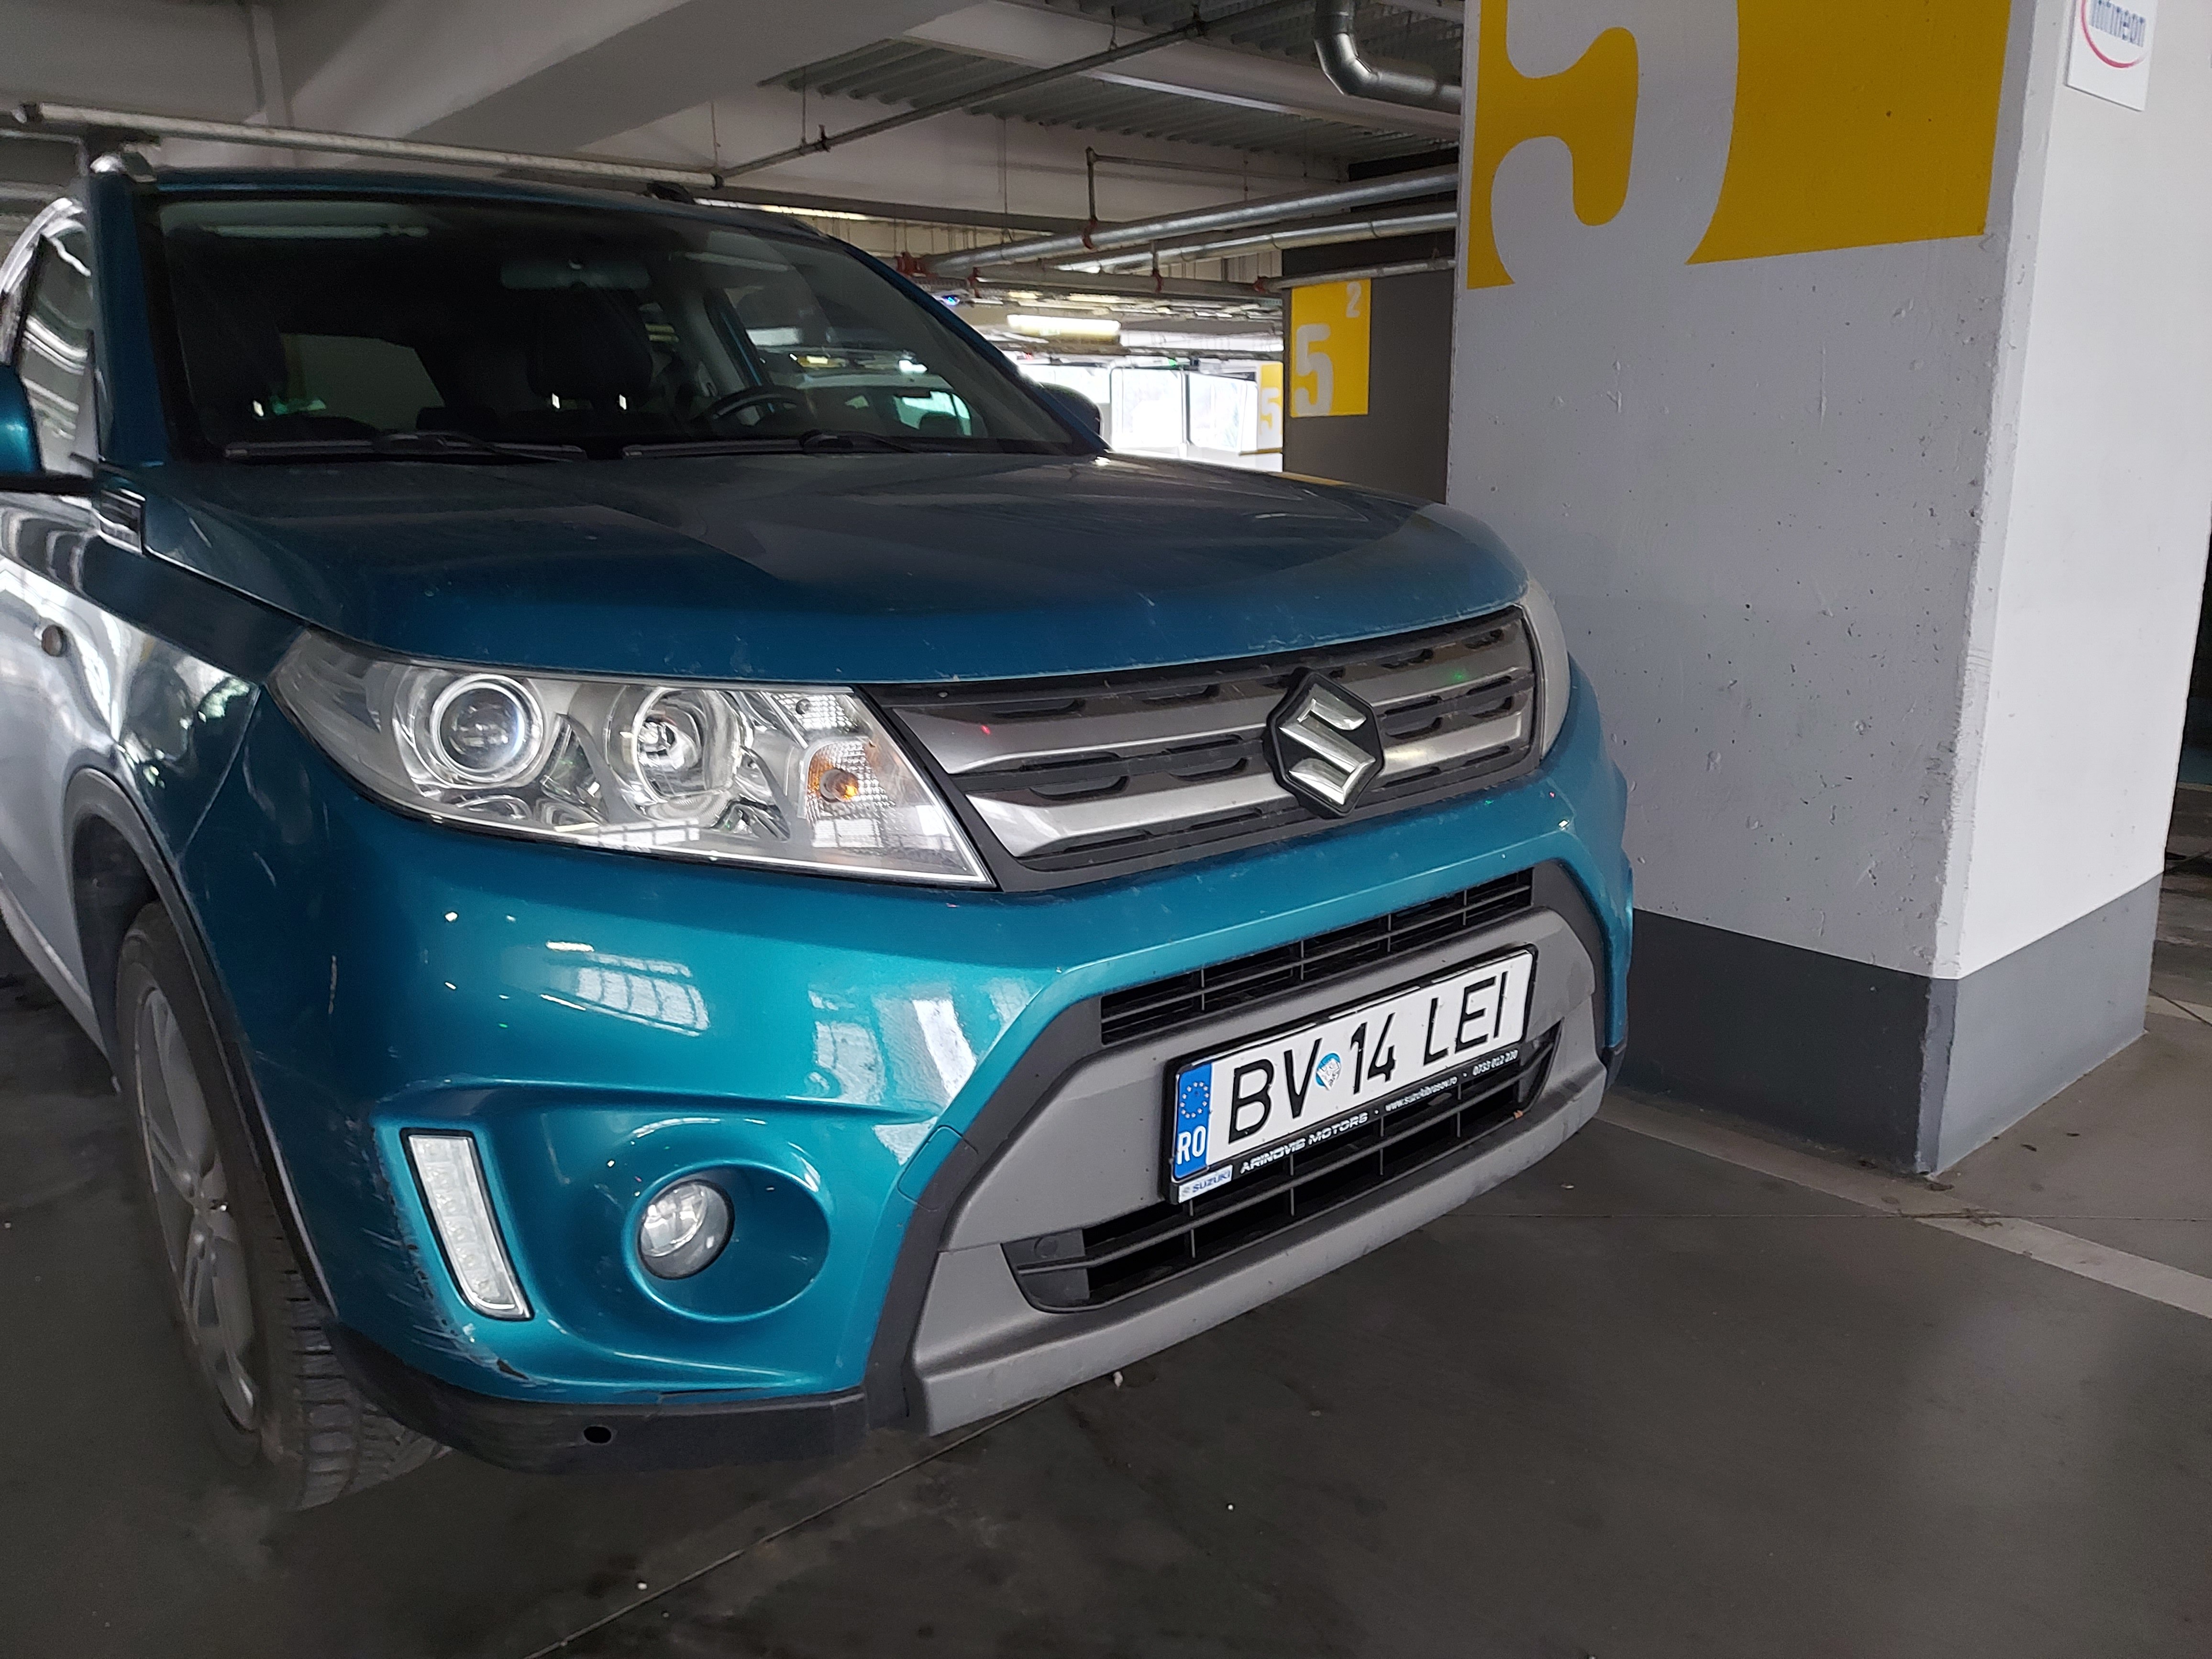
\includegraphics[width=0.4\textwidth]{images/input.jpg}
    \caption{Imaginea de input}
\end{figure}
\FloatBarrier

Pentru început, să analizăm imaginea de input. Un aspect cheie pentru program este poziționarea camerei de fotografiat, care influențează în mod direct încadrarea numărului de înmatriculare în imagine. În fotografia dată, precum și în setul de date pe care a fost testat programul, numărul de înmatriculare este situat în partea inferioară a imaginii, deoarece acesta este amplasat în general în partea de jos a vehiculelor.

Unghiul de fotografiere și distanța de la care se face poza nu influențează semnificativ procesul de segmentare, cel puțin în anumite limite. Deși, în contextul parcărilor auto, camerele de fotografiat de la intrare sunt fixate astfel încât să se obțină imagini clare din unghiuri optime, în acest exemplu, imaginea este surprinsă într-o manieră neobișnuită pentru a înțelege mai bine impactul anumitor algoritmi folosiți asupra imaginii. Acest lucru permite examinarea mai detaliată a modului în care algoritmii programului gestionează imagini cu condiții diverse de captare și încadrate atipic.

Dimensiunile imaginilor reprezintă un aspect esențial pentru performanța programului. În cazul setului de date pe care a fost testată aplicația, lucrăm cu imagini de înaltă calitate, cu o rezoluție de 4624 x 3468 x 3 și un raport de aspect de 4:3. Această dimensiune generează un număr mare de pixeli, peste 48 de milioane, ceea ce are un impact direct asupra timpului de execuție al aplicației.

Având imagini de aceste dimensiuni, este de așteptat să întâmpinăm provocări legate de viteză și eficiență. O soluție practică este redimensionarea imaginii de input la jumătate, ceea ce reduce numărul total de pixeli, menținând totuși o calitate superioară. Prin acest proces, timpul de execuție este îmbunătățit semnificativ, facilitând o procesare mai rapidă și eficientă, fără a sacrifica prea mult din calitatea imaginii. În acest fel, programul poate gestiona seturi de date mari într-un timp mai scurt, permițându-i să fie mai scalabil și să suporte un volum mai mare de procesare fără a compromite rezultatele.

\begin{figure}[h]
    \centering
    \includegraphics[width=0.4\textwidth]{images/resize.jpg}
    \caption{Imaginea redimensionată}
\end{figure}
\FloatBarrier

Pentru a îmbunătăți timpul de execuție și mai mult, putem optimiza procesarea imaginilor concentrându-ne doar pe jumătatea inferioară a acestora. Știind că numărul de înmatriculare este de obicei amplasat în partea inferioară a vehiculului, putem decupa imaginea astfel încât să păstrăm doar jumătatea de jos a acesteia. Eventual, se pot aplica mici decupaje și din părțile laterale pentru a elimina porțiuni care nu conțin informații relevante.

\begin{figure}[h]
    \centering
    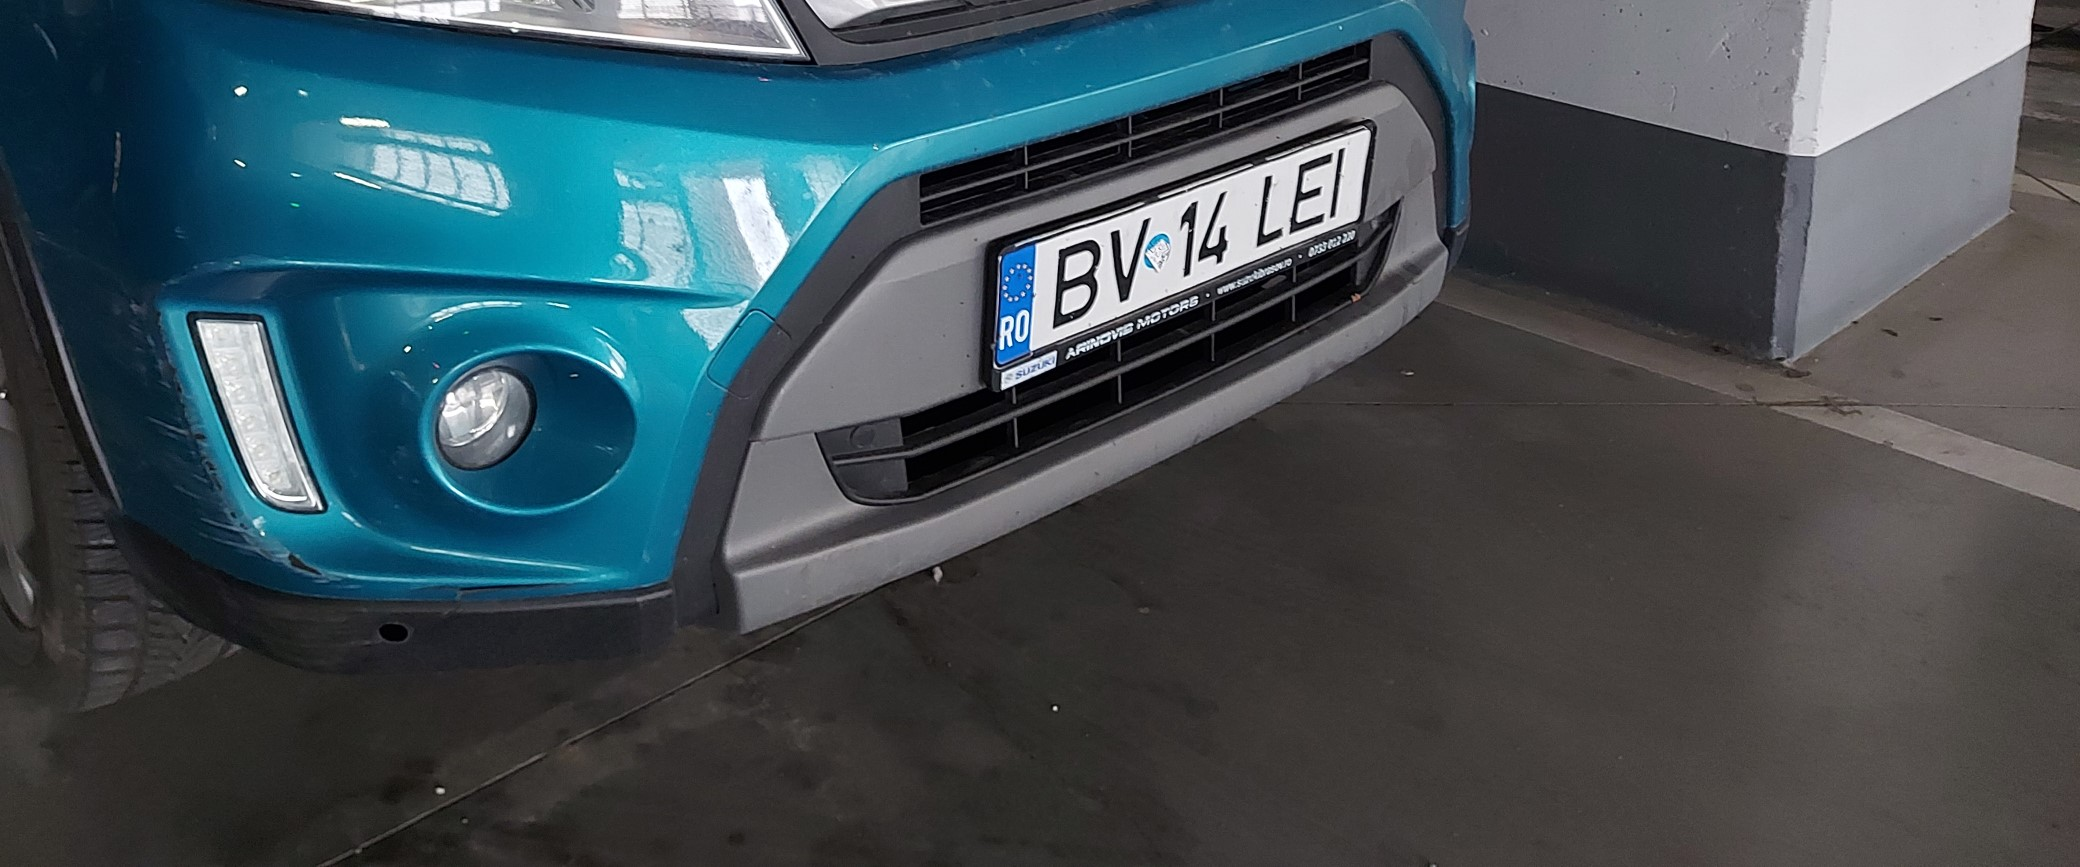
\includegraphics[width=0.4\textwidth]{images/crop.jpg}
    \caption{Partea inferioară din imaginea de input}
\end{figure}
\FloatBarrier

Această decizie are un impact direct asupra numărului de pixeli pe care algoritmii trebuie să-i proceseze, reducându-l considerabil. Cu mai puțini pixeli de analizat, timpul de execuție va fi mai rapid, iar aplicația va fi mai eficientă în procesarea imaginilor. În plus, această strategie poate ajuta la focalizarea algoritmilor pe zonele relevante ale imaginii, eliminând părțile neesențiale și reducând riscul de confuzie sau erori.

După ce imaginea a fost decupată, următorul pas este aplicarea unui filtru Gaussian pentru a elimina zgomotul generat de factori externi. Zgomotul din imagini poate apărea din diverse motive, cum ar fi condițiile de iluminare sau interferențele electronice. Filtrul Gaussian este un instrument eficient pentru reducerea zgomotului și pentru netezirea imaginii, fără a afecta contururile în mod semnificativ.

\begin{figure}[h]
    \centering
    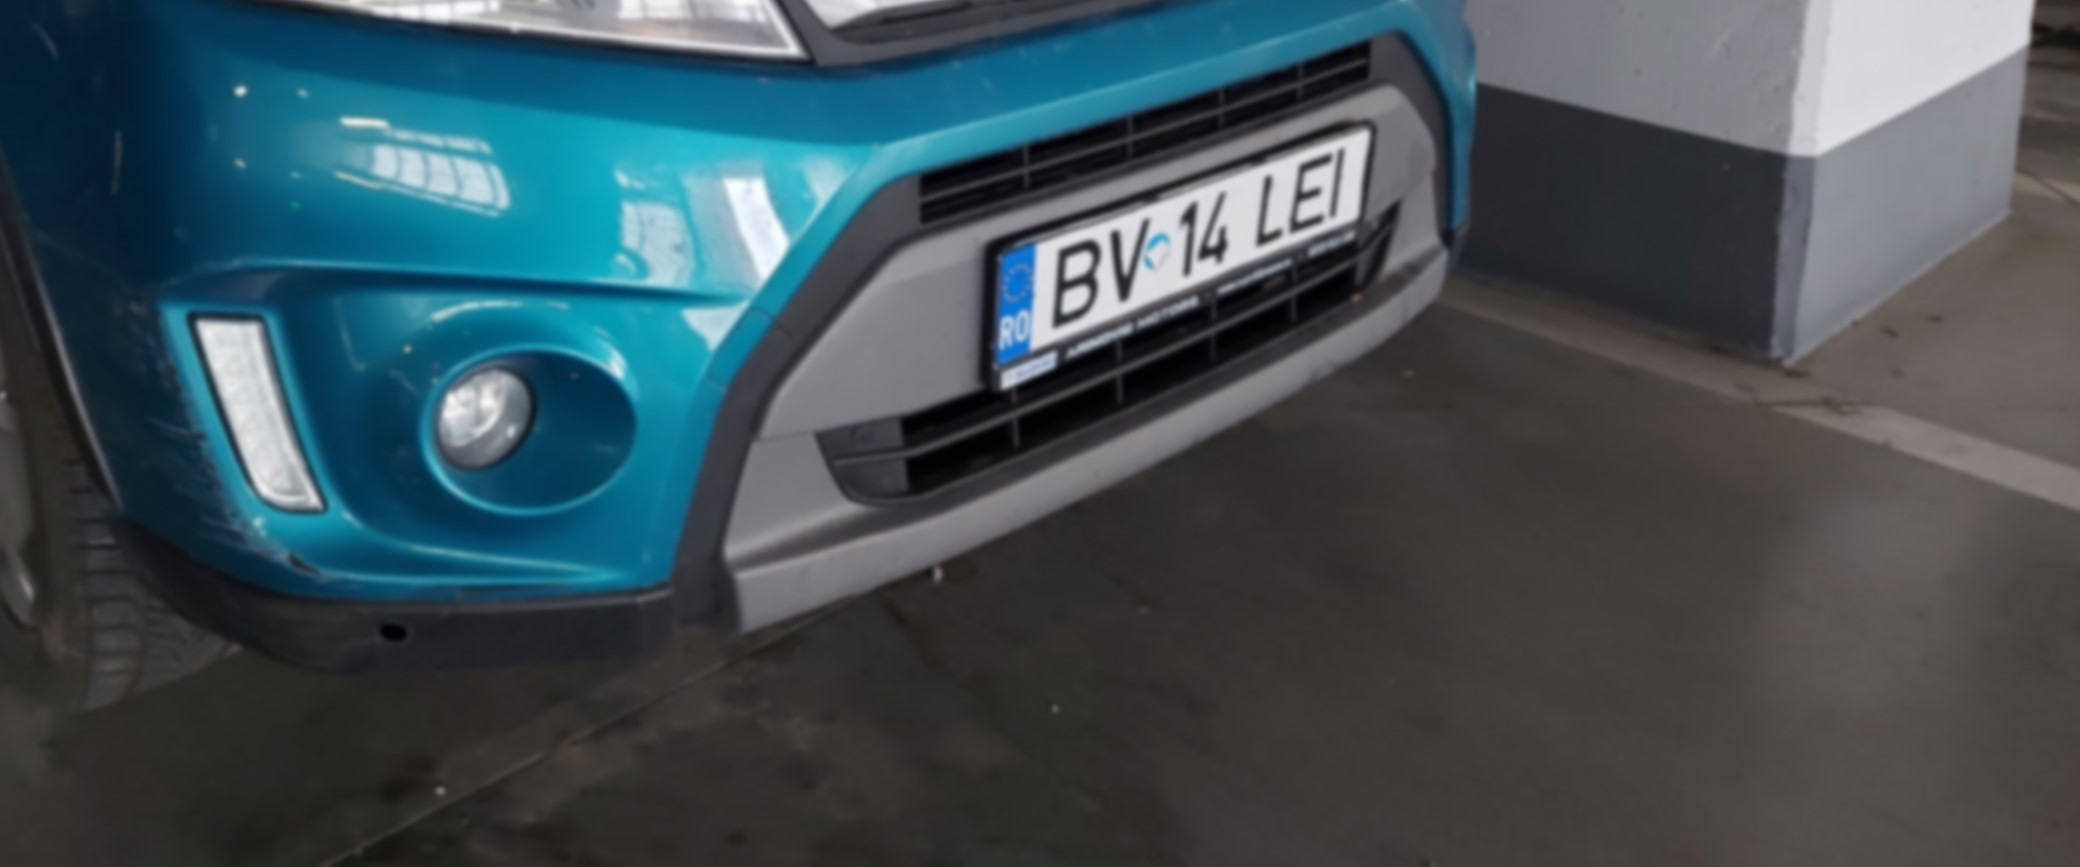
\includegraphics[width=0.4\textwidth]{images/gauss.jpg}
    \caption{Eliminarea zgomotului}
\end{figure}
\FloatBarrier

Cat despre mască, am considerat că una de dimensiune 3 x 3 este suficientă pentru imagine, întrucât nu afectează considerabil contururile așa cum ar face o mască de dimensiuni mai mari, dar totodată elimină o suficientă parte din zgomotul imaginii.

Prin aplicarea acestui filtru, imaginea decupată devine mai curată și mai ușor de procesat de algoritmi, ceea ce contribuie la rezultate mai precise. Contururile rămân clare, facilitând identificarea obiectelor sau a detaliilor importante, în timp ce zgomotul nedorit este redus semnificativ.

În următoarea etapă a procesului de prelucrare a imaginii, un pas esențial în pipeline-ul programului este binarizarea. Scopul este separarea numărului de înmatriculare de restul imaginii, iar una dintre caracteristicile cheie ale unui număr de înmatriculare este culoarea sa, care, în cazul celor din România, este albă.

Imaginile sunt de obicei reprezentate în spațiul de culoare BGR (albastru, verde, roșu), în care culoarea albă are un tuplu de valori de 255 pentru fiecare canal. Totuși, în imagini naturale, factorii externi precum vremea și lumina pot afecta culorile, astfel încât este improbabil să întâlnim albul perfect (255, 255, 255). Pentru a face procesul de binarizare mai robust, putem converti imaginea din BGR în spațiul de culoare HSV (nuanță, saturație, valoare). În acest spațiu, un obiect alb are o saturație scăzută și o valoare ridicată, în timp ce nuanța nu este un factor semnificativ.

\begin{figure}[h]
    \centering
    \begin{minipage}{0.4\textwidth}
        \centering
        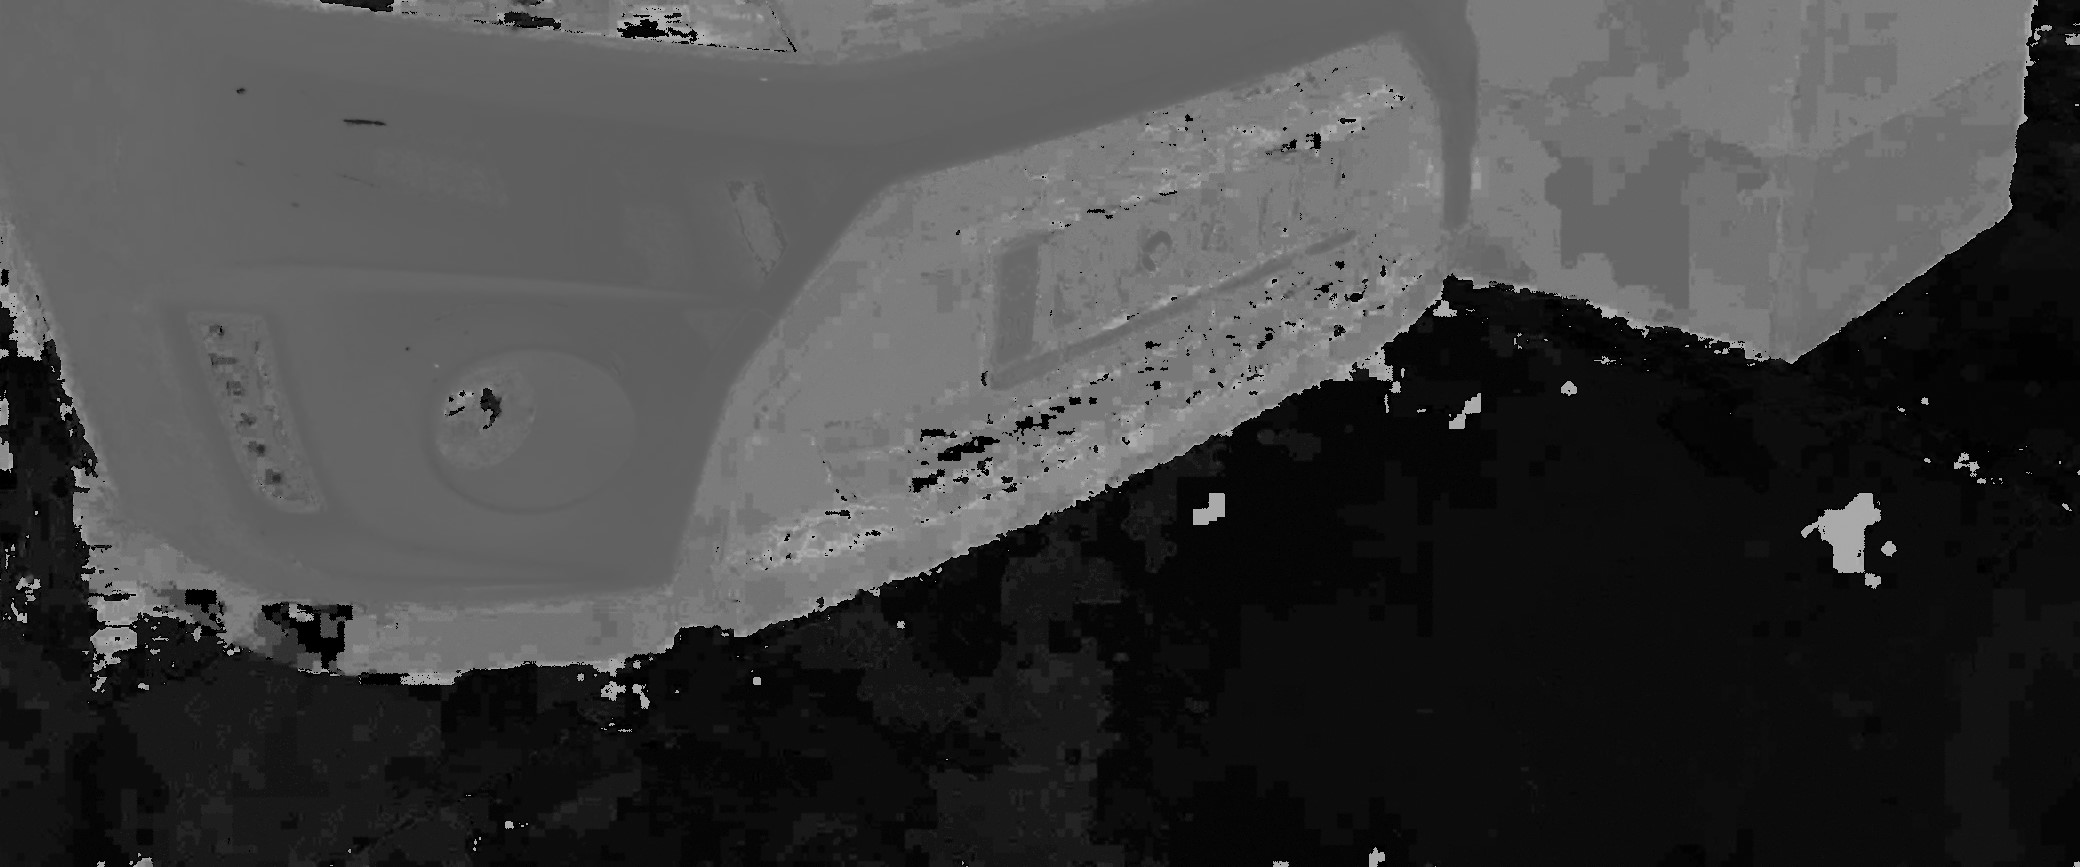
\includegraphics[width=1\textwidth]{images/hue.jpg}
        \caption{Hue (culoare)}
    \end{minipage}
    \hspace{0.05\textwidth}
    \begin{minipage}{0.4\textwidth}
        \centering
        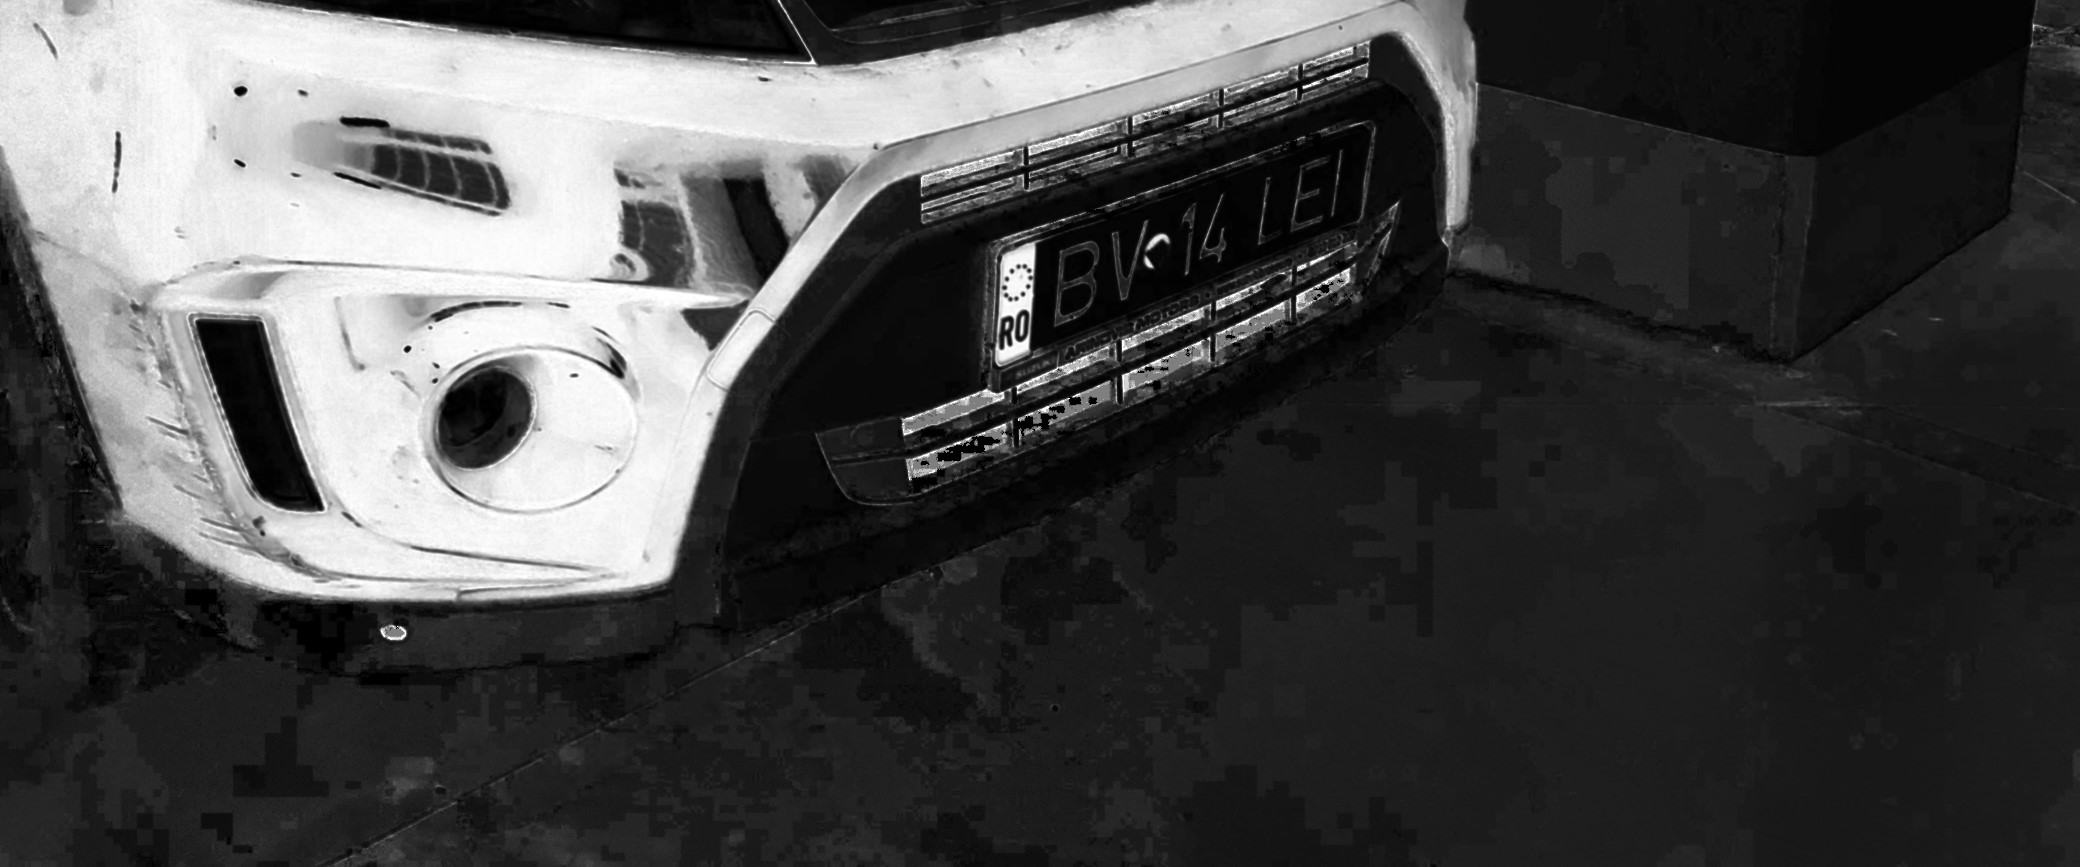
\includegraphics[width=1\textwidth]{images/saturation.jpg}
        \caption{Saturație}
    \end{minipage}
\end{figure}
\begin{figure}[h]
    \centering
    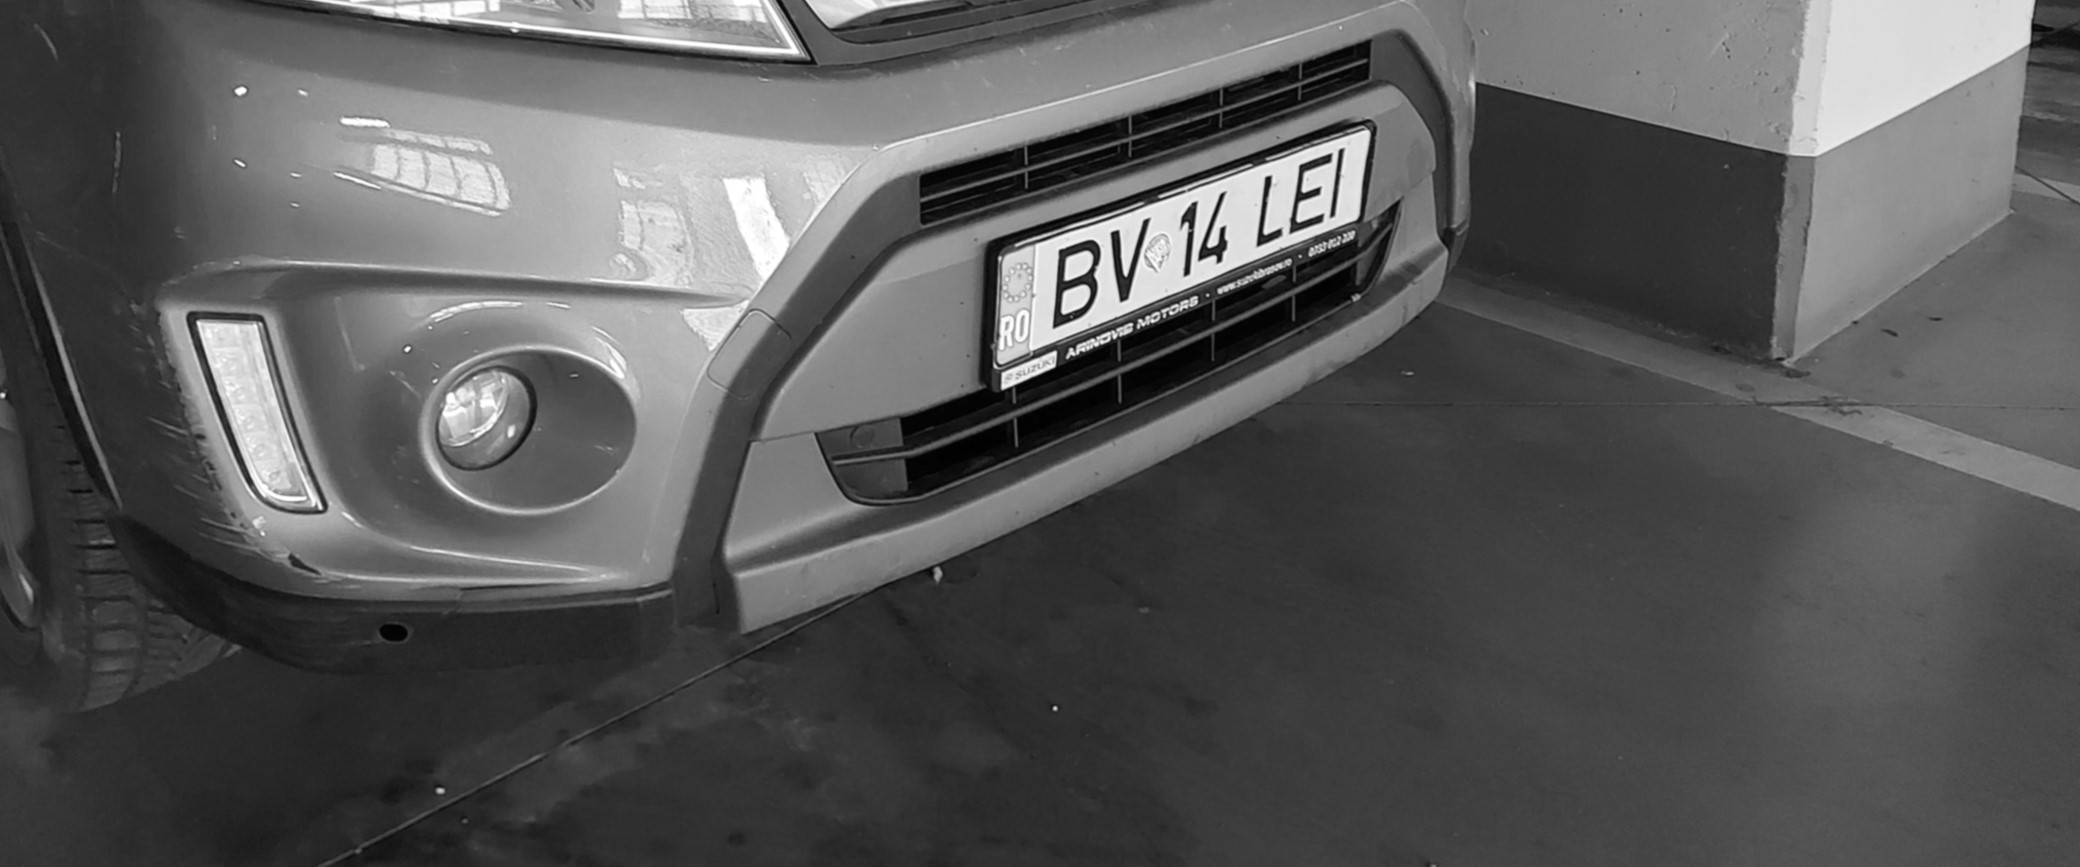
\includegraphics[width=0.4\textwidth]{images/value.jpg}
    \caption{Value (luminozitate)}
\end{figure}
\FloatBarrier

Cu imaginea convertită în spațiul HSV, putem parcurge fiecare pixel și aplica următoarea condiție: dacă pixelul are o saturație scăzută (al doilea canal) și o valoare ridicată (al treilea canal), acesta este considerat ca fiind parte a unui obiect alb, cum ar fi numărul de înmatriculare. În acest caz, pixelul este transformat în alb (255). Dacă nu îndeplinește aceste criterii, este transformat în negru (0). Această abordare creează o imagine binarizată, în care numărul de înmatriculare se va afla într-o regiune albă, față de fundalul imaginii, care va fi negru.

\begin{figure}[h]
    \centering
    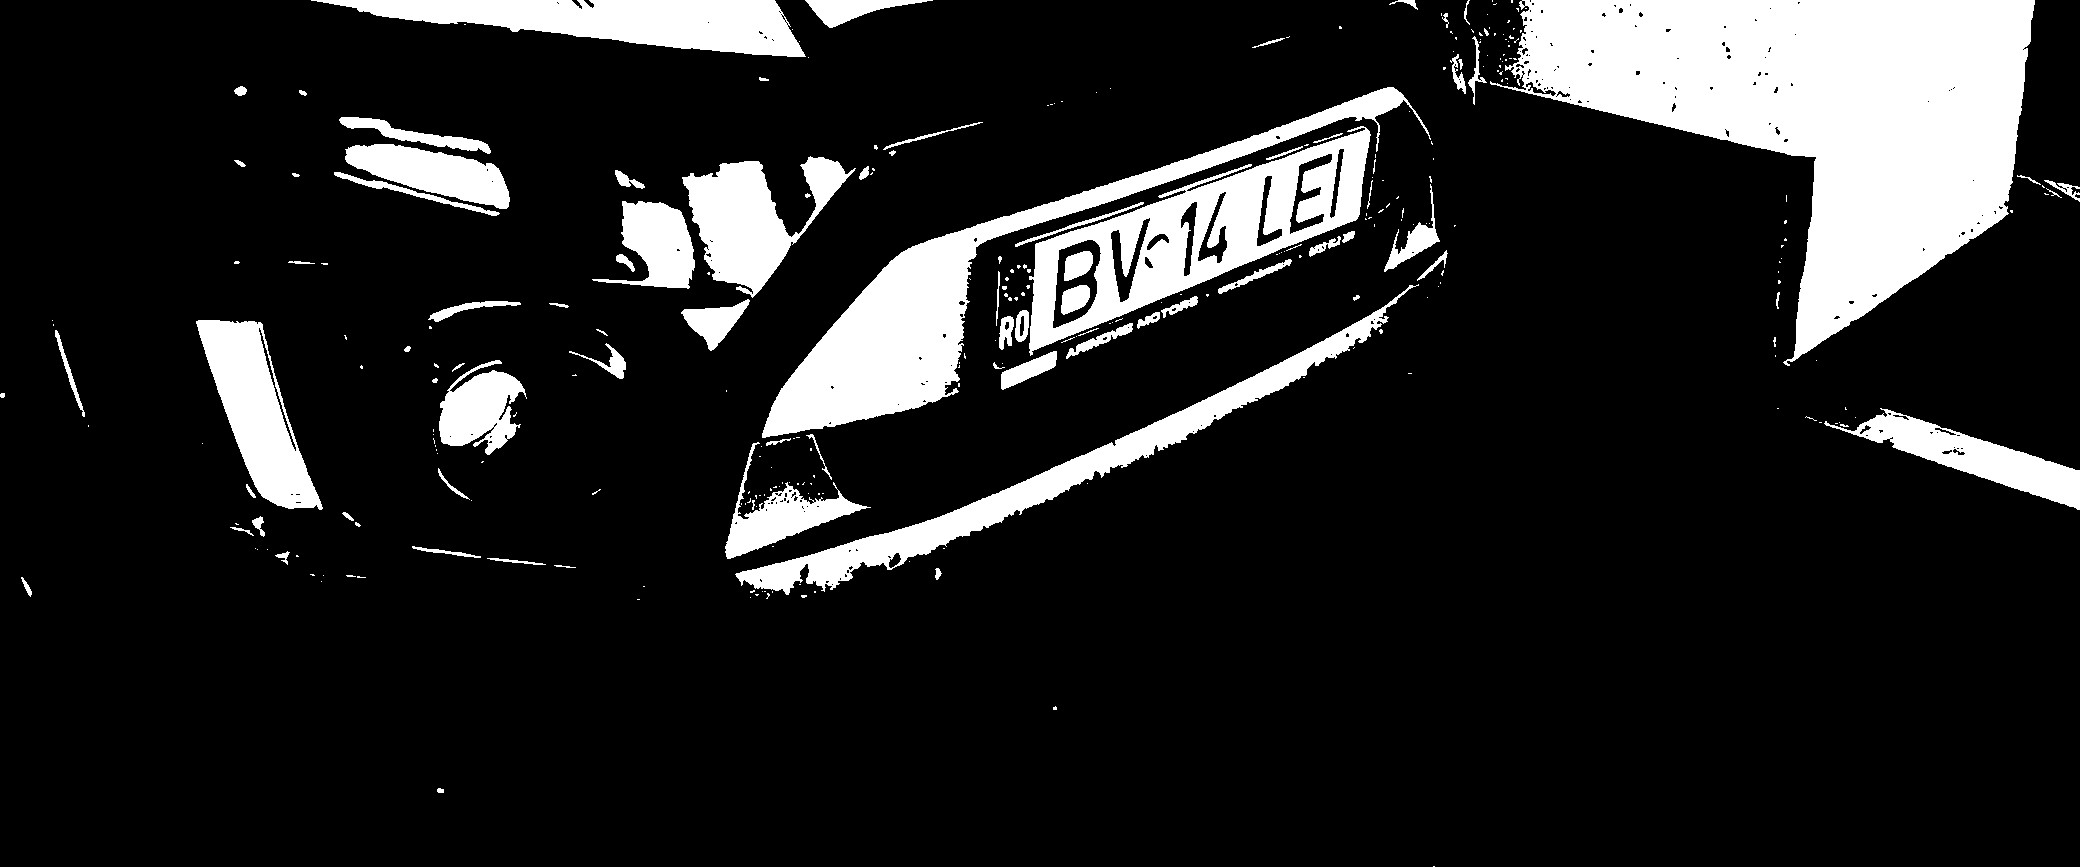
\includegraphics[width=0.4\textwidth]{images/binary.jpg}
    \caption{Imaginea de input cu filtru binar}
\end{figure}
\FloatBarrier

Următorul pas în procesul de analiză a imaginii binarizate este extragerea tuturor componentelor conexe. O componentă conexă este o mulțime de pixeli albi învecinați și conectați între ei, înconjurați la exterior de pixeli negri, cum este și cazul numărului de înmatriculare din imaginea binară. În funcție de valorile stabilite anterior ca praguri la pasul de binarizare, imaginea rezultată va avea mai multe sau mai puține componente conexe. Cu toate acestea, de cele mai multe ori, nu va conține doar componenta căutată, adică numărul de înmatriculare, ci probabil și alte componente conexe nedorite.

\begin{figure}[h]
    \centering
    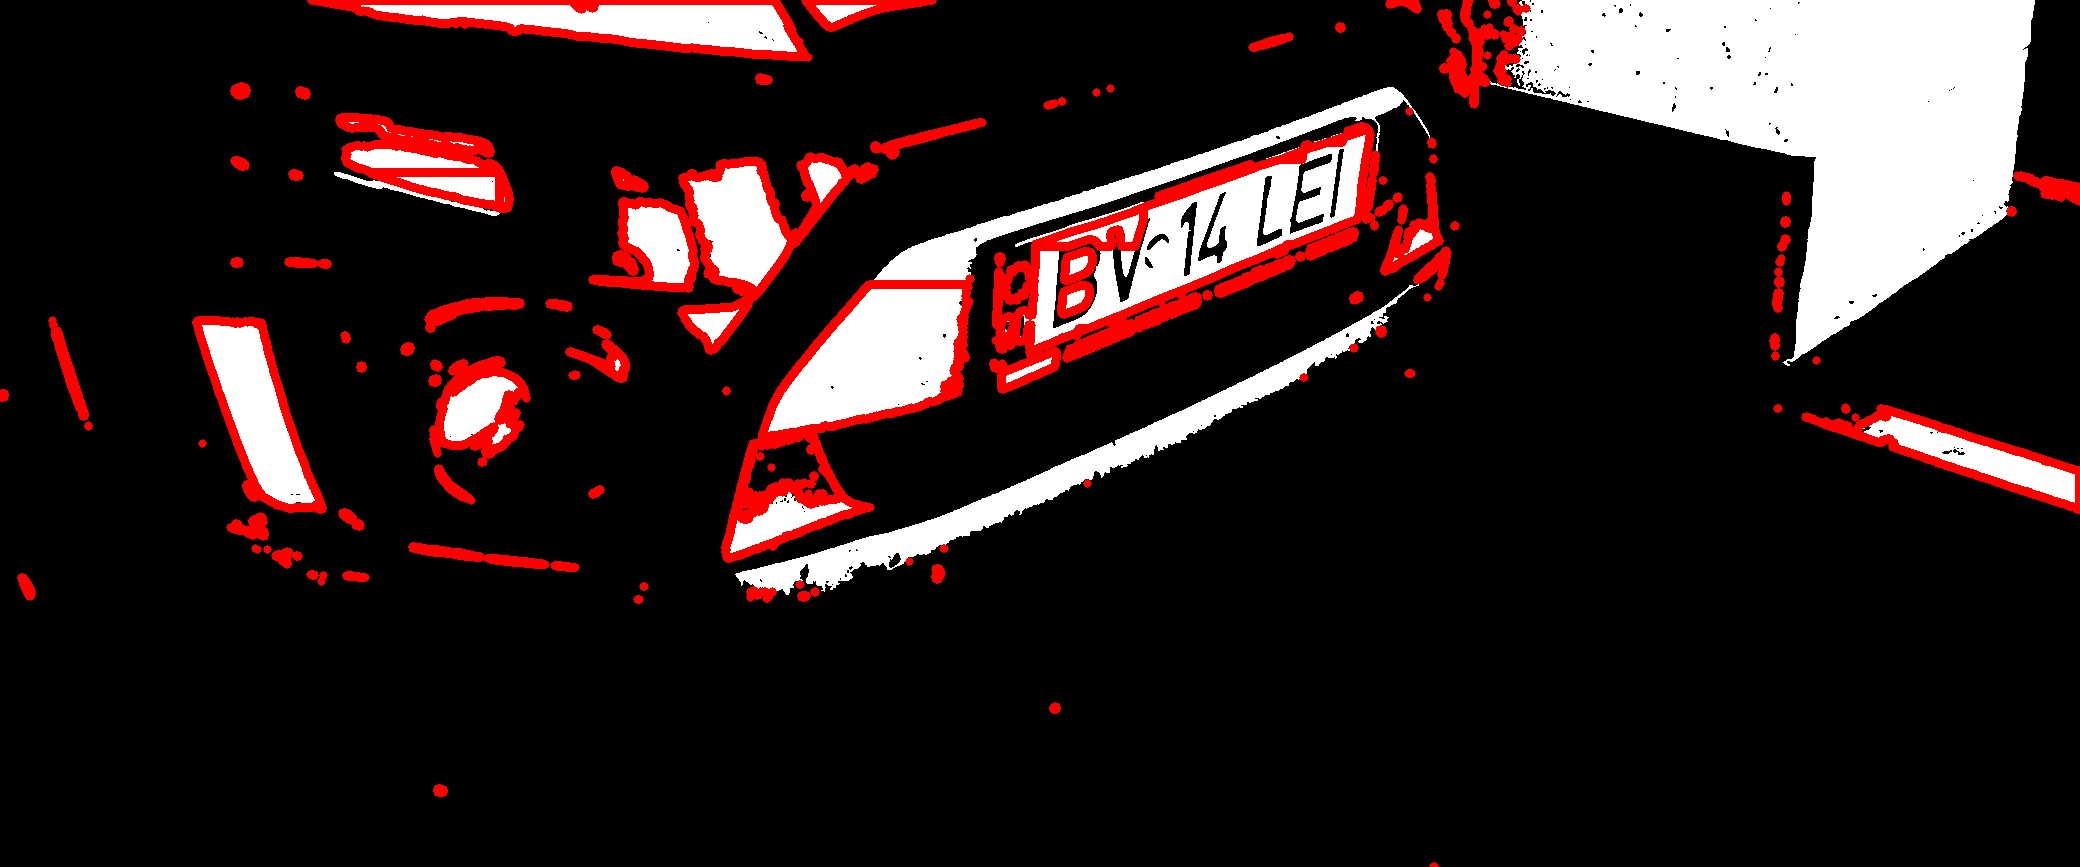
\includegraphics[width=0.4\textwidth]{images/all_connected_components.jpg}
    \caption{Conturul componentelor conexe}
\end{figure}
\FloatBarrier

Pentru a reduce din numărul componentelor conexe, putem utiliza o metodă de filtrare bazată pe dimensiunea ariei. Numărul de înmatriculare, fiind un element semnificativ în imagine, tinde să aibă o arie mai mare în comparație cu alte componente conexe. Prin urmare, putem ordona descrescător toate componentele conexe după dimensiune și să păstrăm doar primele n, unde n este stabilit în funcție de contextul imaginii. În acest exemplu, alegem n = 10, ceea ce înseamnă că rezultatul va fi un vector de dimensiune 10 care conține coordonatele colțului din stânga sus ale fiecărei componente conexe, precum și înălțimea și lățimea fiecărei componente.

\begin{figure}[h]
    \centering
    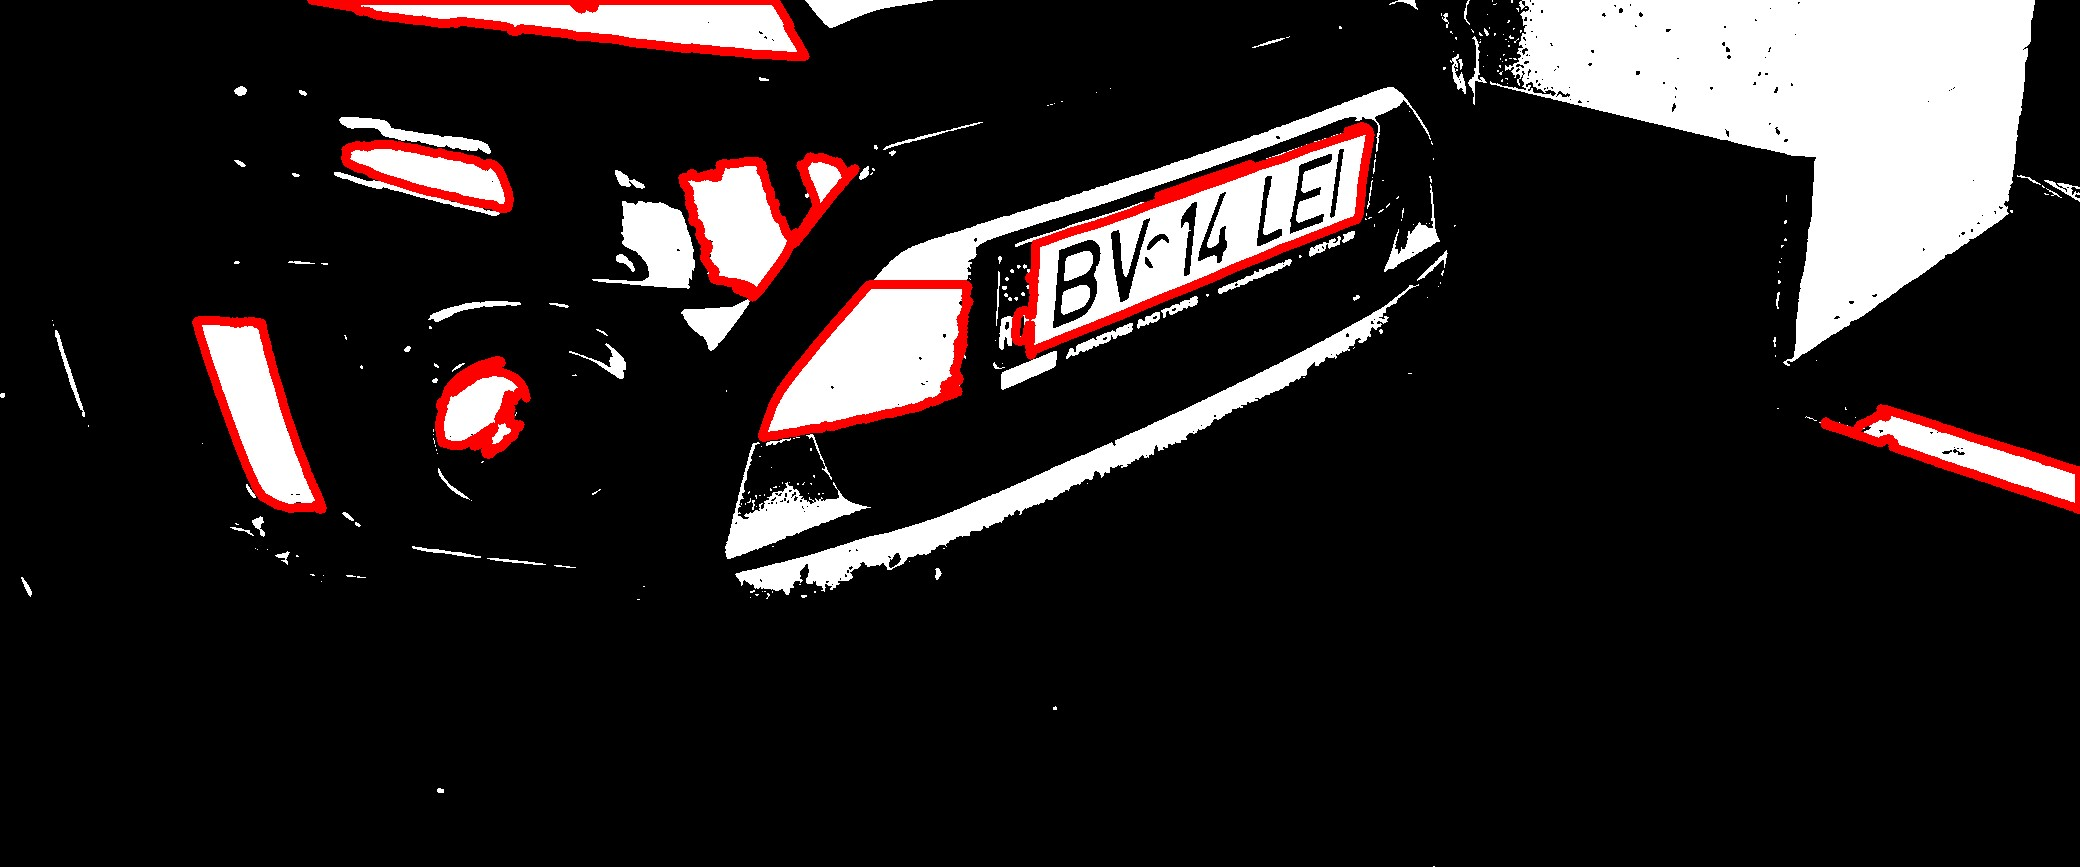
\includegraphics[width=0.4\textwidth]{images/connected_components.jpg}
    \caption{Conturul celor mai mari 10 componente conexe}
\end{figure}
\FloatBarrier

Pentru a identifica componenta conexă ce conține numărul de înmatriculare, vom face segmentări din imagine, numite și regiuni de interes (ROI), pe baza vectorului rezultat, și vom analiza fiecare regiune obținută, care încadrează câte o componentă conexă. Știm că un număr de înmatriculare are o formă dreptunghiulară, cu o înălțime mică în comparație cu lățimea și cu o arie destul de mică în raport cu întreaga imagine. Pe baza acestor informații, putem stabili condiții pentru a filtra componentele conexe și a ne concentra pe cea care ar putea corespunde unui număr de înmatriculare.

\begin{figure}[h]
    \centering
    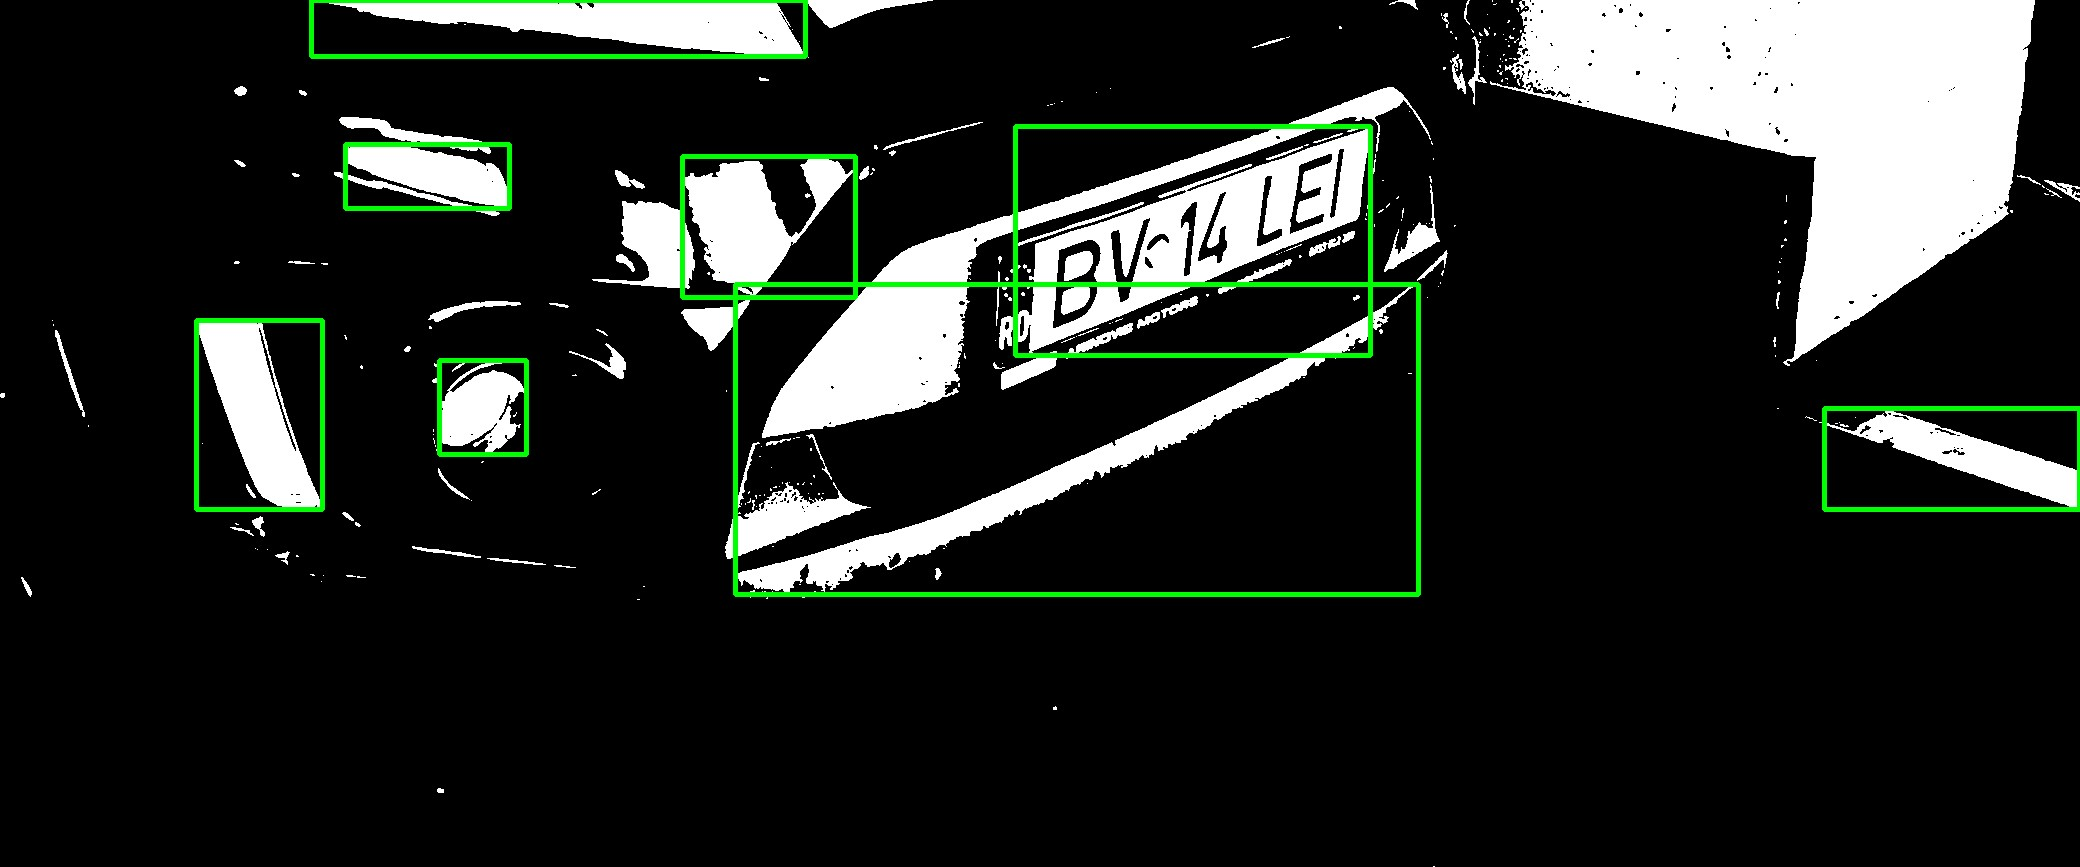
\includegraphics[width=0.4\textwidth]{images/bboxes.jpg}
    \caption{Bounding box-urile componentelor conexe}
\end{figure}
\FloatBarrier

O condiție importantă pentru selecție este raportul dintre înălțimea și lățimea regiunii de interes. Pentru a se califica ca potențial candidat pentru numărul de înmatriculare, înălțimea segmentării trebuie să fie mai mare decât un anumit procent din lățimea acesteia, dar nu mai mare decât un alt procent. De exemplu, putem stabili că înălțimea trebuie să fie între 20\% și 90\% din lățime, permițând o flexibilitate suficientă pentru a include numerele de înmatriculare care ar putea fi înclinate, rezultând forme aproape pătratice.

\[
    ROI.height \in [ROI.width \times min, \ ROI.width \times max]; \, min, \ max \in [0, 1]
\]

Dacă această condiție este îndeplinită, următorul pas este calcularea ariei regiunii de interes și compararea acesteia cu aria totală a imaginii. Pentru a se califica, aria trebuie să fie între anumite limite procentuale, de exemplu, între 1\% și 15\% din aria totală.

\[
    ROI.area \in [Sursa.area \times min, \ Sursa.area \times max]; \, min, \ max \in [0, 1]
\]

Acest proces de filtrare bazat pe aspectul dreptunghiular și dimensiunea ariei ajută la reducerea numărului de componente conexe care nu reprezintă numere de înmatriculare, asigurând că ne concentrăm pe candidații cei mai probabili. În plus, flexibilitatea condițiilor permite ajustări în funcție de imagini cu numere de înmatriculare în poziții variabile sau înclinate.

\begin{figure}[h]
    \centering
    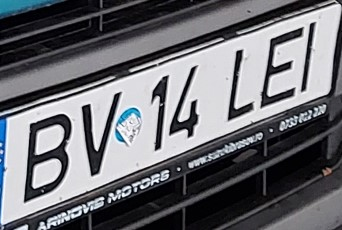
\includegraphics[width=0.4\textwidth]{images/color_roi.jpg}
    \caption{Segmentarea din imaginea de input}
\end{figure}
\FloatBarrier

Acum că regiunea de interes (ROI) pare să aibă dimensiuni similare cu un număr de înmatriculare, putem aplica diferiți algoritmi pentru a detecta contururile, care vor fi folosiți în pașii următori ai programului. Începem prin adăugarea unui padding la regiunea noastră de interes pentru a asigura continuitatea contururilor, evitând astfel întreruperi cauzate de dimensiunile măștilor utilizate pentru detectarea marginilor. Padding-ul este important pentru a ne asigura că niciun pixel relevant nu este omis în zonele limită.

\begin{figure}[h]
    \centering
    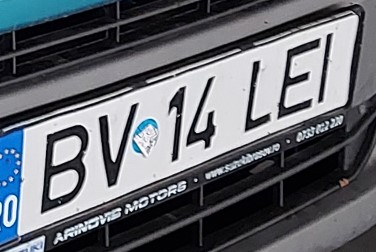
\includegraphics[width=0.4\textwidth]{images/padded_roi.jpg}
    \caption{Imaginea segmentată cu padding adăugat}
\end{figure}
\FloatBarrier

După aceasta, convertim segmentarea în format grayscale, deoarece algoritmii de detectare a marginilor necesită imagini în tonuri de gri.

\begin{figure}[h]
    \centering
    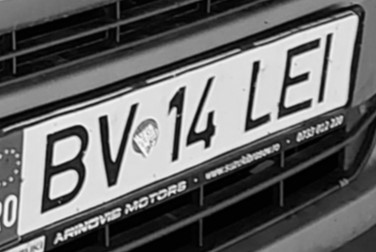
\includegraphics[width=0.4\textwidth]{images/gray_roi.jpg}
    \caption{Imaginea segmentată in format grayscale}
\end{figure}
\FloatBarrier

Primul pas este aplicarea filtrului Sobel, care detectează marginile bazându-se pe derivata imaginii. Pentru a obține o binarizare clară, aplicăm un filtru de binarizare Triangular Thresholding pentru a păstra doar pixelii relevanți detectați de Sobel, care sunt cu adevărat contururi.

\begin{figure}[h]
    \centering
    \begin{minipage}{0.4\textwidth}
        \centering
        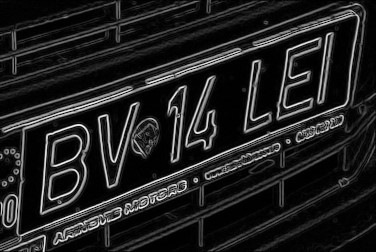
\includegraphics[width=1\textwidth]{images/sobel.jpg}
        \caption{Sobel}
    \end{minipage}
    \hspace{0.05\textwidth}
    \begin{minipage}{0.4\textwidth}
        \centering
        
\includegraphics[width=1\textwidth]{images/binary_sobel.jpg}
        \caption{Sobel cu filtru binar}
    \end{minipage}
\end{figure}
\FloatBarrier

Pentru a ne asigura că am captat toți pixelii relevanți din imagine, aplicăm și un filtru de obținere a gradientului morfologic tot pe regiunea în format grayscale, urmat de încă un filtru de binarizare Triangular Thresholding. Astfel, avem două imagini binare: una cu rezultatele filtrului Sobel și alta cu gradientul morfologic.

\begin{figure}[h]
    \centering
    \begin{minipage}{0.4\textwidth}
        \centering
        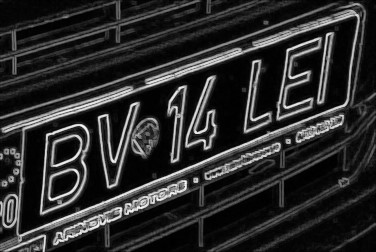
\includegraphics[width=1\textwidth]{images/gradient.jpg}
        \caption{Gradienții morfologici}
    \end{minipage}
    \hspace{0.05\textwidth}
    \begin{minipage}{0.4\textwidth}
        \centering
        
\includegraphics[width=1\textwidth]{images/binary_gradient.jpg}
        \caption{Gradienții morfologici cu filtru binar}
    \end{minipage}
\end{figure}
\FloatBarrier

Următorul pas este combinarea acestor două imagini binare, păstrând în imaginea cu gradienții morfologici doar acei pixeli care apar în cel puțin una dintre imaginile binare.

\begin{figure}[h]
    \centering
    \begin{minipage}{0.4\textwidth}
        \centering
        
\includegraphics[width=1\textwidth]{images/or_binary.jpg}
        \caption{Reuniunea celor doua imagini binare (masca)}
    \end{minipage}
    \hspace{0.05\textwidth}
    \begin{minipage}{0.4\textwidth}
        \centering
        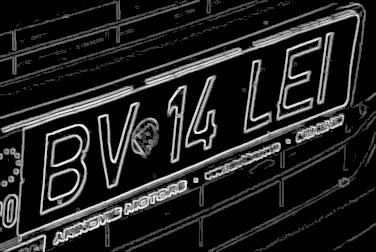
\includegraphics[width=1\textwidth]{images/or_gradient.jpg}
        \caption{Gradienții morfologici dupa mască}
    \end{minipage}
\end{figure}
\FloatBarrier

Acum, că avem doar pixelii care ar putea aparține unor contururi, aplicăm un filtru de subțiere Non-Maximum Suppression pentru a obține margini de un pixel grosime, astfel încât contururile să fie clare și precise.

\begin{figure}[h]
    \centering
    
\includegraphics[width=0.4\textwidth]{images/non_maximum_suppression.jpg}
    \caption{Edge map de un pixel grosime}
\end{figure}
\FloatBarrier

În următorul pas, revenim la regiunea de interes în formatul grayscale și aplicăm un filtru de binarizare automatizat, cum ar fi Triangle Thresholding sau Otsu. Segmentarea este un dreptunghi în care ar trebui să fie inclus numărul de înmatriculare (dacă este regiunea corectă), dar în acesta pot exista și alte elemente din imaginea inițială care nu ne interesează.

\begin{figure}[h]
    \centering
    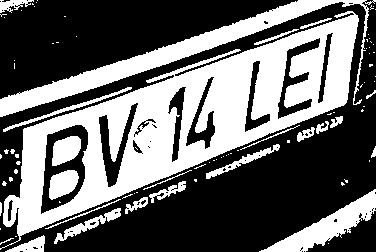
\includegraphics[width=0.4\textwidth]{images/before_roi.jpg}
    \caption{Imaginea segmentată cu filtru binar}
\end{figure}
\FloatBarrier

După aplicarea filtrului de binarizare, în imagine ar trebui observat un chenar alb care conține literele și cifrele numărului de înmatriculare și care ar trebui să fie separat de restul imaginii. Acum putem căuta din nou componentele conexe și păstra strict pe cea de dimensiunea cea mai mare, care ar trebui să fie chenarul alb. Însă pot apărea situații în care această binarizare este eronată și chenarul alb este conectat cu alte zone formate din pixeli albi.

Pentru a corecta acest lucru, folosim edge map-ul obținut anterior. Știm că în edge map contururile sunt reprezentate ca pixeli de valoare 255, deci putem verifica că pixelii albi (255) din edge map sunt negri (0) în regiunea binarizată. Acest lucru asigură că pixelii contururilor rămân separați și nu conectează eronat zonele între ele.

\begin{figure}[h]
    \centering
    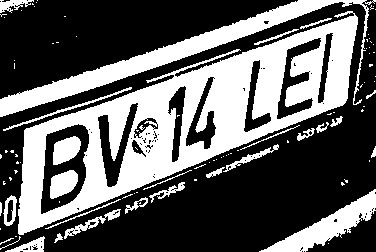
\includegraphics[width=0.4\textwidth]{images/after_roi.jpg}
    \caption{Corecția imaginii segmentate}
\end{figure}
\FloatBarrier

Pentru a fi complet siguri că nu există legături incorecte, putem aplica o operație morfologică de tip Opening. Această operație separă obiectele legate incorect prin linii fine.

După operația de Opening, este posibil să apară noi componente conexe, deci aplicăm din nou căutarea componentelor conexe și păstrăm doar componenta de dimensiunea cea mai mare. Aceasta ar trebui să fie chenarul alb care conține numărul de înmatriculare.

\begin{figure}[h]
    \centering
    
\includegraphics[width=0.4\textwidth]{images/roi.jpg}
    \caption{Regiunea textului}
\end{figure}
\FloatBarrier

Pentru a reduce numărul de segmente și pentru a ne apropia de regiunea care conține numărul de înmatriculare, putem adăuga o nouă condiție pentru imaginea segmentată, care ar trebui să conțină numai zona textului numărului de înmatriculare. Această condiție stabilește că înălțimea zonei respective ar trebui să fie aproape egală cu întreaga înălțime a imaginii de segmentare. Prin urmare, putem compara înălțimea acestei zone cu un procentaj, să zicem 80\%, din înălțimea regiunii de interes pentru a valida corectitudinea segmentării.

\[
    width > ROI.width \times percent; \, percent \in [0, 1]
\]

În pasul de rectificare, trebuie să obținem 4 coordonate pe baza cărora se va face rectificarea, aceste 4 coordonate fiind chiar colțurile chenarului alb în care se află numărul de înmatriculare. Pentru început, scădem din imaginea sursă imaginea sursă erodată pentru a obține exact conturul chenarului alb. Pe imaginea rezultată putem aplica algoritmul Hough, care ne va returna liniile din imagine, din intersectarea cărora putem obține coordonatele colțurilor.

\begin{figure}[h]
    \centering
    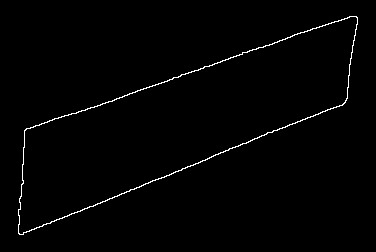
\includegraphics[width=0.4\textwidth]{images/edges.jpg}
    \caption{Conturul regiunii}
\end{figure}
\FloatBarrier

Pentru a face acest lucru, primul pas este să stabilim parametrii funcției Hough. Doi parametri importanți din funcția Hough sunt lungimea minimă admisă pentru o linie ca aceasta să fie adăugată ca rezultat și distanța maximă dintre două linii ca acestea să fie considerate de fapt aceeași linie, dar cu o întrerupere eronată între ele, și astfel în vectorul rezultat, în loc de două linii, să fie adăugată una singură formată din aceste două. Valorile acestor doi parametri sunt obținute în mod automatizat pe baza bounding box-ului rotit.

\begin{figure}[h]
    \centering
    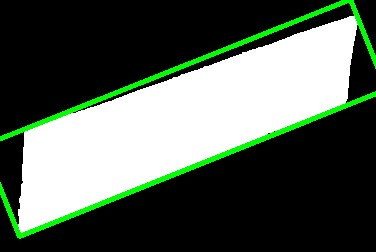
\includegraphics[width=0.4\textwidth]{images/rotated_rect.jpg}
    \caption{Bounding box-ul rotit al regiunii}
\end{figure}
\FloatBarrier

Având acest bounding box în care componenta conexă este încadrată exact, putem estima dimensiunile acesteia, deci și dimensiunile liniilor Hough. Astfel, pentru lungimea minimă a liniilor și distanța maximă dintre acestea, vom considera anumite procente din înălțimea bounding box-ului. Totuși, aceste procente pot fi destul de mici, de exemplu, 30\% pentru lungimea minimă a liniilor și 15\% pentru distanța maximă dintre acestea.

Această abordare este necesară deoarece, cu cât unghiul de fotografiere este mai inclinat, cu atât și numărul de înmatriculare va fi mai înclinat în imagine. În astfel de cazuri, algoritmul Hough, în loc să detecteze puține linii de dimensiuni mari, detectează multe linii de dimensiuni mici. Astfel, dacă stabilim valori mari parametrilor funcției, multe linii nu vor fi luate în calcul când numărul de înmatriculare este mai inclinat. Chiar și așa, dacă în continuare nu am obținut toate liniile de care aveam nevoie, putem decrementa treptat lungimea minimă a acestora, pentru a obține în final mai multe linii.

\begin{figure}[h]
    \centering
    
\includegraphics[width=0.4\textwidth]{images/lines.jpg}
    \caption{Liniile Hough}
\end{figure}
\FloatBarrier

Liniile de care avem nevoie sunt câte una din fiecare parte a chenarului alb, mai exact partea de sus, jos, stânga, dreapta, pentru că mai apoi să le putem găsi punctele de intersectie. Însă, algoritmul Hough nu ne oferă și informația de care parte aparține fiecare linie, așa că următoarea etapă este o sortare. Pentru început, vom sorta liniile ca fiind verticale sau orizontale. Putem obține această informație în funcție de panta fiecărei drepte:

\[
    slope = \frac{y_2 - y_1}{x_2 - x_1}
\]

Unghiul de înclinare se calculează apoi astfel:

\[
    angle = \lvert \arctan(slope) \times \frac{180}{\pi} \rvert
\]

Deci, dacă unghiul este aproape de 0 grade, linia este considerată orizontală, iar dacă este aproape de 90 de grade, linia este considerată verticală. Trebuie să ținem cont și de cazurile în care panta este complet verticală, pentru a evita împărțirea la zero.

\begin{figure}[h]
    \centering
    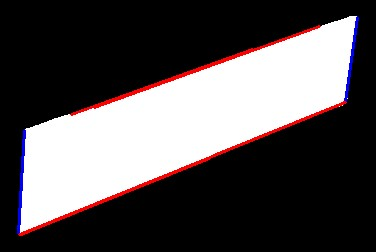
\includegraphics[width=0.4\textwidth]{images/horizontal_vertical_lines.jpg}
    \caption{Separarea liniilor verticale și orizontale}
\end{figure}
\FloatBarrier

După sortarea liniilor în verticale și orizontale, putem identifica liniile de care avem nevoie pentru fiecare parte a chenarului alb: partea de sus, jos, stânga, dreapta. Pentru a face acest lucru, luăm ca referință o linie verticală și una orizontală prin centrul imaginii, față de care se compară și se clasifică fiecare linie detectată de algoritmul Hough.

\begin{figure}[h]
    \centering
    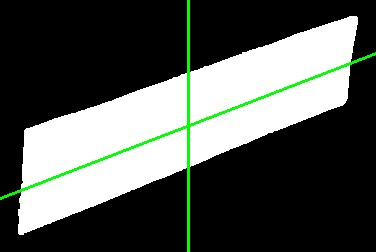
\includegraphics[width=0.4\textwidth]{images/reference_lines.jpg}
    \caption{Liniile de comparație}
\end{figure}
\FloatBarrier

În trasarea celor două linii de referință, vom ține cont și de pante, cel puțin în cazul celei orizontale, deoarece numărul de înmatriculare poate fi inclinat la un unghi atât de mare încât unele linii să fie clasificate eronat. În cazul în care numărul de înmatriculare este inclinat la un anumit unghi, și liniile trasate prin centrul imaginii trebuie să fie inclinate la unghiul respectiv pentru a se face clasificarea într-un mod corect.

După ce avem vectorii cu liniile orizontale și verticale, putem să-i parcurgem și să comparăm fiecare linie cu liniile de referință pentru a determina orientarea lor. Linia verticală de referință este utilizată pentru a compara liniile verticale, iar linia orizontală de referință pentru cele orizontale.

Pentru a face această comparație, putem folosi formula distanței dintre două drepte:

\[
    distance = (x - x_1) \cdot (y_2 - y_1) - (y - y_1) \cdot (x_2 - x_1)
\]

Semnul distanței ajută să separăm liniile detectate. Cele de deasupra liniei de referință vor avea distanțe pozitive, iar cele de dedesubt vor avea distanțe negative. La fel, liniile din dreapta vor avea distanțe pozitive față de linia de referință verticală, iar cele din stânga vor avea distanțe negative.

\begin{figure}[h]
    \centering
    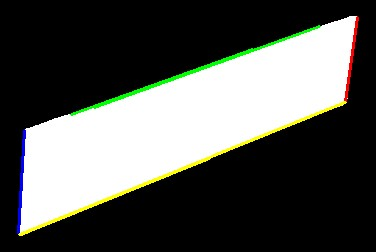
\includegraphics[width=0.4\textwidth]{images/multiple_lines.jpg}
    \caption{Clasificarea Liniile Hough}
\end{figure}
\FloatBarrier

Ideal, rezultatul ar trebui să fie compus din patru linii, câte una pentru fiecare parte a chenarului alb. Cu toate acestea, din cauza erorilor de detectare sau a înclinațiilor, pot apărea mai multe segmente în loc de o singură linie. Dacă avem mai multe segmente, putem căuta capetele cele mai îndepărtate în funcție de orientare pentru a le lega între ele și a obține o singură linie pentru fiecare parte.

\begin{figure}[h]
    \centering
    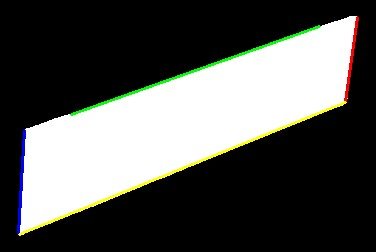
\includegraphics[width=0.4\textwidth]{images/sorted_lines.jpg}
    \caption{Cele 4 linii rezultate}
\end{figure}
\FloatBarrier

Acesta este și momentul în care verificăm dacă trebuie să aplicăm din nou algoritmul Hough cu parametrii ajustați sau dacă am găsit toate liniile necesare. Dacă avem cele patru linii căutate, pasul următor este să calculăm punctele de intersecție între ele pentru a obține coordonatele colțurilor chenarului alb. Ordinea este următoarea:
\begin{itemize}[itemsep=5pt, parsep=0pt]
    \item Punctul din stânga sus se obține prin intersectarea liniei din stânga cu cea de sus.
    \item Punctul din dreapta sus se obține prin intersectarea liniei din dreapta cu cea de sus.
    \item Punctul din dreapta jos se obține prin intersectarea liniei din dreapta cu cea de jos.
    \item Punctul din stânga jos se obține prin intersectarea liniei din stânga cu cea de jos.
\end{itemize}

\begin{figure}[h]
    \centering
    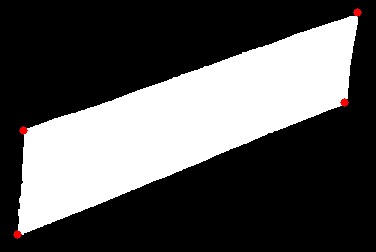
\includegraphics[width=0.4\textwidth]{images/points.jpg}
    \caption{Punctele de rectificare}
\end{figure}
\FloatBarrier

O problemă des întâlnită cu liniile detectate este că punctele de intersecție pot fi în afara imaginii, ceea ce necesită un padding suficient de mare pentru a cuprinde toate cele patru puncte de intersecție. Pentru a rezolva această situație, trebuie să căutăm coordonatele cele mai mici și cele mai mari pentru X și Y dintre punctele calculate anterior:

\[
    \begin{aligned}
        minX & = ROI.width, \, minY = ROI.height, \ maxX = 0, \, maxY = 0,
    \end{aligned}
\]
Pentru fiecare punct (\(x, y\)):
\[
    \begin{aligned}
        minX & = \min(minX, x); \\
        minY & = \min(minY, y); \\
        maxX & = \max(maxX, x); \\
        maxY & = \max(maxY, y).
    \end{aligned}
\]

După ce avem aceste valori, putem calcula dimensiunea padding-ului necesar pentru fiecare parte a imaginii. Dacă punctele de intersecție sunt în afara imaginii, vom ajusta padding-ul pentru a le include:

\[
    \begin{aligned}
        paddingRight  & = \max(0, maxX - (src.cols - 1)), \\
        paddingBottom & = \max(0, maxY - (src.rows - 1)), \\
        paddingLeft   & = \max(0, -minX),                 \\
        paddingTop    & = \max(0, -minY).
    \end{aligned}
\]

Această abordare ne permite să ajustăm imaginea astfel încât toate punctele de intersecție să fie incluse în limitele acesteia, inclusiv punctele care au coordonate mai mari decât dimensiunile imaginii inițiale. Însă, dacă există și puncte cu coordonate negative pentru care a fost adăugat padding în partea de sus a imaginii sau în partea din stânga, suntem nevoiți să ajustăm toate punctele de intersecție cu valoarea padding-ului adăugat pentru a reflecta noua poziție în cadrul imaginii extinse:

Pentru fiecare punct (\(x, y\)):
\[
    \begin{aligned}
        x = paddingLeft + x, \\
        y = paddingTop + y.
    \end{aligned}
\]

Acum că avem cele patru coordonate ale colțurilor chenarului alb și ne-am asigurat că sunt în interiorul imaginii, putem trece la pasul de rectificare. Rectificarea presupune transformarea geometrică a regiunii de interes pentru a alinia numărul de înmatriculare într-o poziție corectă, obținând astfel o imagine rectificată.

Pentru a începe procesul de rectificare, calculăm dimensiunile imaginii rezultate. Pentru a determina înălțimea corectă a numărului de înmatriculare, scădem coordonata Y a punctului din stânga sus din coordonata Y a punctului din stânga jos:

\[
    height = DownLeft.y - UpLeft.y
\]

Pentru a obține lățimea, folosim raportul cunoscut pentru numărul de înmatriculare, unde lățimea este de 4.3 ori mai mare decât înălțimea:

\[
    width = 4.3 \times height
\]

Cu aceste dimensiuni calculate, putem stabili punctele corespunzătoare pentru fiecare colț al chenarului alb în imaginea destinată. Ordinea punctelor pentru colțurile chenarului alb este: stânga sus, dreapta sus, dreapta jos, stânga jos. Pentru imaginea rectificată, punctele corespondente vor fi:

\begin{itemize}[itemsep=5pt, parsep=0pt]
    \item (0, 0) pentru stânga sus,
    \item (width - 1, 0) pentru dreapta sus,
    \item (width - 1, height - 1) pentru dreapta jos,
    \item (0, height - 1) pentru stânga jos
\end{itemize}

\begin{figure}[h]
    \centering
    
\includegraphics[width=0.4\textwidth]{images/points_on_black.jpg}
    \caption{Punctele de rectificare in imaginea destinație}
\end{figure}
\FloatBarrier

Cu aceste puncte corespondente, putem calcula matricea de transformare utilizând funcția de transformare geometrică. Aplicând această transformare pe imaginea segmentată în formatul grayscale, obținem în final numărul de înmatriculare într-o formă rectificată.

\begin{figure}[h]
    \centering
    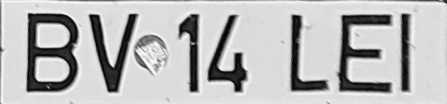
\includegraphics[width=0.4\textwidth]{images/transformed.jpg}
    \caption{Imaginea rectificată}
\end{figure}
\FloatBarrier

Imaginea rezultată ar trebui să conțină literele și cifrele numărului de înmatriculare pe fundal alb. Însă, există și situații în care rectificarea nu este tocmai ideală, iar astfel pot apărea diverse probleme: anumite caractere nu sunt în totalitate incadrate în imagine, iar astfel, spre exemplu, un caracter este ușor tăiat într-o parte anume, sau, în cazul opus, zona rectificată este ușor mai mare și astfel se obțin detalii în plus la extremitățile imaginii, detalii ce nu sunt necesare.

Ca o primă soluție este decuparea de pe fiecare parte a imaginii a câte o linie sau a câte o coloană, ca mai apoi să se adauge un padding alb în locul liniilor și coloanelor decupate. Decupând o mică parte din imagine, se reduce din posibila zonă care este în plus. De asemenea, padding-ul alb de jur împrejurul imaginii asigură că nu va exista un contur discontinuu al chenarului alb, cum s-ar întâmpla în cazul în care o literă nu este întru totul încadrată în imagine și întrerupe conturul dreptunghiular al chenarului.

\begin{figure}[h]
    \centering
    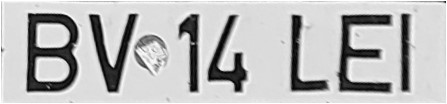
\includegraphics[width=0.4\textwidth]{images/boardered.jpg}
    \caption{Imaginea rectificată cu padding adăugat}
\end{figure}
\FloatBarrier

Următorul pas este aplicarea unui filtru Binary Thresholding pe imaginea rectificată. Acest lucru va crea o imagine binarizată în care literele și cifrele numărului de înmatriculare vor fi separate de fundal. Însă, se aplică și un filtru de inversare a culorilor deoarece caracterele sunt de culoare neagră pe un fundal alb, pe când acestea ar trebui să fie albe pe un fundal negru.

\begin{figure}[h]
    \centering
    
\includegraphics[width=0.4\textwidth]{images/text.jpg}
    \caption{Imaginea rectificată cu filtru binar}
\end{figure}
\FloatBarrier

Caracterele numărului de înmatriculare pot fi considerate și componente conexe în imaginea binară. De asemenea, știm că numerele de înmatriculare în formatul din România au între 6 și 8 caractere, deci tot atâtea componente conexe trebuie să existe în imaginea binară. Însă, nu este întotdeauna așa, căci uneori numărul de înmatriculare poate avea diferite însemnări pe care le vom considera artefacte și pe care dorim să le eliminăm.

O primă etapă este detectarea tuturor componentelor conexe din imagine și ordonarea acestora după aria lor. Cele mai mari componente conexe tind să fie caracterele numărului de înmatriculare. După ordonare, păstrăm primele opt componente, deoarece, așa cum am stabilit, un număr de înmatriculare nu are mai mult de opt caractere.

\begin{figure}[h]
    \centering
    
\includegraphics[width=0.4\textwidth]{images/before_denoise.jpg}
    \caption{Primele 8 componente conexe}
\end{figure}
\FloatBarrier

Cu toate acestea, tot este posibil ca una sau două componente conexe din imagine să fie de fapt zgomot. Pentru a detecta și elimina posibilul zgomot, putem folosi înălțimea ca un factor comun între caractere. Calculăm înălțimea mediană a componentelor conexe și o folosim ca referință pentru a compara înălțimea fiecărei componente cu cea mediană:

\[
    \left| median - height \right| > median \times percent; \, percent \in [0, 1]
\]

Dacă diferența dintre înălțimea componentei conexe curente și cea mediană este mai mare decât un anumit procent din înălțimea mediană, de exemplu 20\%, putem considera acea componentă ca fiind zgomot și se elimină. Prin aplicarea acestui filtru bazat pe înălțime, ne putem asigura că imaginea finală conține doar componentele conexe care corespund literelor și cifrelor numărului de înmatriculare.

\begin{figure}[h]
    \centering
    
\includegraphics[width=0.4\textwidth]{images/after_denoise.jpg}
    \caption{Eliminarea componentelor conexe eronate}
\end{figure}
\FloatBarrier

De asemenea, ca la un pas anterior, pentru a fi complet siguri că nu există legături incorecte între componentele conexe, putem aplica și o operație morfologică de tip Opening. Această operație separă obiectele legate incorect prin linii fine.

După operația de Opening, este posibil să apară noi componente conexe, motiv pentru care se aplică din nou funcția descrisă anterior și astfel se elimină noile componente conexe, care nu sunt caractere, rezultate din urma operației morfologice.

În urma aplicării tuturor tehnicilor de procesare a imaginilor, am obținut o imagine în care textul numărului de înmatriculare arată ca și cum ar fi fost tastat manual într-un fișier. Aceasta este o imagine potrivită pentru modelul de recunoaștere a caracterelor Tesseract OCR. Totuși, pentru a obține rezultate mai bune, este util să furnizăm modelului AI fiecare caracter separat, pe rând.

Pentru a realiza acest lucru, aplicăm pe imaginea binară rectificată funcția implementată într-un pas anterior ce detectează componentele conexe, pentru a obține bounding box-urile tuturor caracterelor. Rezultatul este din nou un vector ce conține coordonatele colțului din stânga sus ale fiecărui bounding box, precum și înălțimea și lățimea fiecărei componente. Este important să cunoaștem ordinea corectă a caracterelor în imagine pentru a putea reconstrui textul numărului de înmatriculare din caracterele recunoscute.

\begin{figure}[h]
    \centering
    
\includegraphics[width=0.4\textwidth]{images/chars.jpg}
    \caption{Bounding box-urile caracterelor}
\end{figure}
\FloatBarrier

Cu toate acestea, ordinea în care componentele conexe sunt stocate în vector poate să nu coincidă cu ordinea reală a caracterelor în imagine. Pentru a remedia acest lucru, sortăm vectorul în ordine crescătoare după coordonata X a fiecărui bounding box. Astfel, obținem o ordine a componentelor conexe care corespunde ordinii reale a caracterelor din imagine.

Știm că numerele de înmatriculare care respectă formatul din România conțin una sau două litere, urmate de două sau trei cifre, și încheiate cu alte trei litere. Această structură ne poate ajuta să îmbunătățim recunoașterea caracterelor. În următoarea etapă, vom partitiona caracterele numărului de înmatriculare în trei regiuni.

Deși știm numărul total de caractere din imagine, primele două regiuni ale numărului de înmatriculare pot avea un număr variabil de caractere, ceea ce înseamnă că nu știm exact unde se termină prima regiune și începe a doua. Pentru a determina acest lucru, trebuie să calculăm distanțele dintre colțurile bounding box-urilor vecine și să identificăm distanța cea mai mare, deoarece aceasta va fi între prima și a doua regiune a numărului de înmatriculare.

Odată ce am identificat cea mai mare distanță între componentele conexe, putem partitiona caracterele în funcție de regiuni:

\begin{itemize}[itemsep=5pt, parsep=0pt]
    \item Prima regiune: cuprinde toate componentele conexe de la început până la cea dinaintea distanței calculate.
    \item A doua regiune: începe de la componenta conexă imediat după distanța cea mai mare și se întinde până la componenta conexă dinaintea ultimelor trei.
    \item A treia regiune: include ultimele trei componente conexe, începând de la antepenultima și terminând cu ultima.
\end{itemize}

Intr-un final, se memoreaza indexul de început pentru fiecare regiune.

\begin{figure}[h]
    \centering
    
\includegraphics[width=0.4\textwidth]{images/partitioned.jpg}
    \caption{Clasificarea caracterelor}
\end{figure}
\FloatBarrier

Tesseract OCR poate primi ca input imaginea binară cu textul complet și apoi i se pot specifica zonele pentru recunoașterea caracterelor, bazându-ne pe bounding box-uri. Cu toate acestea, bounding box-urile nu includ spațiu pentru padding, ceea ce este esențial pentru model AI. De aceea, vom segmenta fiecare caracter din imagine conform bounding box-urilor și îi vom adăuga padding.

Numărul de linii și coloane pentru padding poate fi calculat automat, folosind un procent din dimensiunile bounding box-ului. Vom considera un procent semnificativ, cum ar fi 60\%. Prin înmulțirea acestui procent cu înălțimea și lățimea bounding box-ului, putem determina numărul de linii și coloane care trebuie adăugate în jurul imaginii segmentate pentru a oferi suficient spațiu:

\[
    \begin{aligned}
        paddingX & = BBox.width \times percent  \\
        paddingY & = BBox.height \times percent
    \end{aligned}
\]

Însă, înainte de a adăuga padding fiecărui caracter, este necesar să actualizăm informațiile legate de bounding box. Dimensiunile padding-ului trebuie adăugate la dimensiunile inițiale ale bounding box-ului, de două ori, deoarece padding-ul este aplicat pe ambele părți ale imaginii, atât pe axa X, cât și pe axa Y:

\[
    \begin{aligned}
        BBox.width  & = BBox.width + paddingX \times 2,  \\
        BBox.height & = BBox.height + paddingY \times 2,
    \end{aligned}
\]

Revenim la bounding box-urile inițiale, pe baza cărora vom realiza segmentările în imaginea binară pentru a extrage fiecare caracter. Din bounding box-uri cu padding-ul asociat, putem extrage valoarea specifică a padding-ului pentru fiecare caracter și apoi o putem adăuga la imaginea segmentată.

După ce toate caracterele segmentate sunt obținute, fiecare având padding-ul adăugat, următorul pas este concatenarea lor într-un singur șir, recreând astfel textul inițial cu această nouă distanțare.

Va trebui să generăm, de asemenea, o imagine complet neagră de dimensiuni suficient de mari pentru a cuprinde toate caracterele, împreună cu padding-ul lor. În primul rând, vom determina înălțimea acesteia, care va fi echivalentă cu înălțimea celui mai înalt bounding box. Lățimea va fi calculată ca suma tuturor lățimilor bounding box-urilor.

Anterior, am ajustat dimensiunile bounding box-urilor pentru a se potrivi cu padding-ul, însă acum trebuie să modificăm și colțurile acestora. Coordonata X a fiecărui bounding box poate fi calculată ca suma lățimilor bounding box-urilor anterioare acestuia, iar coordonata Y poate fi calculată ca diferența dintre înălțimea imaginii și înălțimea bounding box-ului, împărțită la 2, pentru a centra caracterul pe axa Y:

\[
    \begin{aligned}
        width & = 0,
    \end{aligned}
\]
Pentru fiecare bounding box:
\[
    \begin{aligned}
        y     & = \frac{height - BBox.height}{2}, \\
        x     & = width,                          \\
        width & = width + BBox.width.
    \end{aligned}
\]

Din acest punct, revenim la segmentele realizate anterior pentru fiecare caracter și le inserăm, pe rând, în imaginea complet neagră generată anterior, conform noilor bounding box-uri.

\begin{figure}[h]
    \centering
    
\includegraphics[width=0.4\textwidth]{images/spaced.jpg}
    \caption{Spațierea caracterelor}
\end{figure}
\FloatBarrier

Acum, cunoscând atât bounding box-urile cu padding, cât și cele fără padding, putem folosi indicii obținuți anterior pentru a separa aceste bounding box-uri în funcție de regiunile de care aparțin.

Pe baza acestor indici, se pot impune condiții suplimentare pentru a ne asigura că segmentarea imaginii originale conține într-adevăr numărul de înmatriculare. Se verifică dacă al doilea indice este egal cu 2 sau 3, deoarece s-a stabilit că prima regiune poate avea maximum două caractere. De asemenea, se verifică dacă intervalul dintre al doilea și al treilea indice conține exact două sau trei caractere.

Următorul pas implică utilizarea modelului AI Tesseract OCR pentru recunoașterea textului în imagine. Se creează o instanță de tip tesseract::TessBaseAPI și se dezactivează toate dicționarele implicite, deoarece acestea nu sunt necesare în acest context. Se setează și un whitelist care indică dacă modelul trebuie să caute litere sau cifre, în funcție de regiunea în care se află caracterul dintre cele trei regiuni obținute anterior.

Modelului i se oferă ca input imaginea binară cu caracterele distanțate și se parcurg, pe rând, fiecare dintre bounding box-uri pentru a specifica zonele în care să se recunoască textul.

\begin{figure}[h]
    \centering
    
\includegraphics[width=0.4\textwidth]{images/input_ocr.jpg}
    \caption{Bounding box-urile caracterelor cu padding adăugat (input-uri OCR) }
\end{figure}
\FloatBarrier

Dacă în segmentul de imagine nu a fost recunoscut niciun caracter sau au fost recunoscute mai multe, se decrementează dimensiunea bounding box-ului și se încearcă din nou recunoașterea, sperând că de această dată să fie identificat caracterul corect. Decrementarea continuă până când bounding box-ul revine la dimensiunile inițiale, încadrând caracterul cu precizie minimă.

\[
    \begin{aligned}
        x      & = x - 1,      \\
        y      & = y - 1,      \\
        width  & = width - 2,  \\
        height & = height - 2.
    \end{aligned}
\]

\begin{figure}[h]
    \centering
    
\includegraphics[width=0.4\textwidth]{images/output_ocr.jpg}
    \caption{Decrementarea bounding box-urilor până la recunoaștere corectă a caracterelor}
\end{figure}
\FloatBarrier

Dacă totuși bounding box-ul a revenit la dimensiunile inițiale și modelul AI nu a reușit să recunoască caracterul din imagine, este posibil ca problema să fie cauzată de litera "I". În anumite cazuri, Tesseract OCR nu recunoaște acest caracter, așa că se utilizează o tehnică de Template matching pentru a determina dacă respectivul caracter nerecunoscut este "I" sau nu.

\begin{figure}[h]
    \centering
    
\includegraphics[height=0.2\textwidth]{images/i.jpg}
    \caption{Segmentarea literei nerecunoscute}
\end{figure}
\FloatBarrier

În pasul de template matching, se va încărca în program o imagine template pentru litera "I".

\begin{figure}[h]
    \centering
    
\includegraphics[height=0.2\textwidth]{images/template.jpg}
    \caption{Template-ul literei "I"}
\end{figure}
\FloatBarrier

Pentru început, redimensionăm această imagine template la dimensiunile caracterului segmentat. Vom calcula raportul de aspect pentru imaginea template și noua lățime pe care o va avea:

\[
    \begin{aligned}
        aspectRation   & = Template.width / Template.height, \\
        Template.width & = Sursa.height * aspectRadion.
    \end{aligned}
\]

Pe imaginea redimensionată, se aplică un filtru de tip "Binary Thresholding" pentru a obține regiunea exactă a literei.

\begin{figure}[h]
    \centering
    
\includegraphics[height=0.2\textwidth]{images/binary_template.jpg}
    \caption{Template-ul literei "i" cu filtru binar}
\end{figure}
\FloatBarrier

În acest moment, litera poate fi înconjurată neuniform de linii și coloane negre, motiv pentru care dorim să o extragem din imaginea inițială și să creăm o imagine în care litera să aibă un spațiu uniform pe toate laturile. Astfel, se caută contururile în imagine pentru a identifica conturul singurei regiuni albe existente, care reprezintă litera. Pe baza acestui contur, se extrage litera din imagine și se inserează într-o imagine complet neagră cu dimensiuni egale cu cele ale literei, dar cu un padding de o unitate pe toate laturile.

Deși template-ul a fost redimensionat la înălțimea segmentării, din cauza uniformizării padding-ului, este posibil ca dimensiunea să nu rămână cea stabilită inițial. Prin urmare, vom calcula diferența dintre aceste două înălțimi pentru a obține padding-ul suplimentar care trebuie adăugat la șablon în partea de sus și de jos. Această diferență se împarte la jumătate pentru a adăuga aceeași cantitate de padding pe fiecare parte a imaginii. De asemenea, se verifică dacă această diferență este pară, deoarece, în caz contrar, va trebui incrementat padding-ul pe una dintre părți:

\[
    \begin{aligned}
        firstPadding  & = \frac{Sursa.height - Template.height}{2},               \\
        secondPadding & = firstPadding,                                           \\
        secondPadding & = \text{secondPadding} + 1,                               \\
                      & \text{dacă } (Sursa.height - Template.height) \mod 2 = 1.
    \end{aligned}
\]

Pentru a stabili si lățimea imaginii template, se va adăuga un padding similar cu cel anterior, calculat pe baza diferenței dintre lățimea imaginii sursă și lățimea imaginii template. La fel ca înainte, diferența se împarte la jumătate pentru a determina padding-ul care trebuie adăugat de fiecare parte a șablonului si se verifică dacă diferența este pară, astfel încât padding-ul să fie distribuit uniform:

\[
    \begin{aligned}
        firstPadding  & = \frac{Sursa.width - Template.width}{2},               \\
        secondPadding & = firstPadding,                                         \\
        secondPadding & = \text{secondPadding} + 1,                             \\
                      & \text{dacă } (Sursa.width - Template.width) \mod 2 = 1.
    \end{aligned}
\]

Acum că cele două imagini sunt ajustate la aceeași dimensiune si cu litera "I" reprezentată central după adăugarea padding-ului, se realizează intersectarea celor două regiuni albe utilizând operația logică 'și'.

\begin{figure}[h]
    \centering
    
\includegraphics[height=0.2\textwidth]{images/intersection.jpg}
    \caption{Intersecția celor doua imagini}
\end{figure}
\FloatBarrier

Scorul Dice poate fi calculat pe baza acestei intersecții, indicând cât de mult se suprapun cele două regiuni. Dacă scorul obținut este semnificativ, de exemplu cel puțin 80\%, se poate concluziona că respectivul caracterul nerecunoscut este 'I'. În caz contrar, se consideră că segmentarea inițială nu reprezintă numărul de înmatriculare și se continuă cu următoarea iterație.

În ultima etapă, se compune textul numărului de înmatriculare folosind caracterele recunoscute, se calculează o medie a nivelului de încredere pe baza tuturor scorurilor de încredere obținute pentru fiecare caracter, se memorează data și ora curente, iar în imaginea sursă se desenează un chenar care încadrează numărul de înmatriculare, pe baza segmentării inițiale.

\begin{figure}[h]
    \centering
    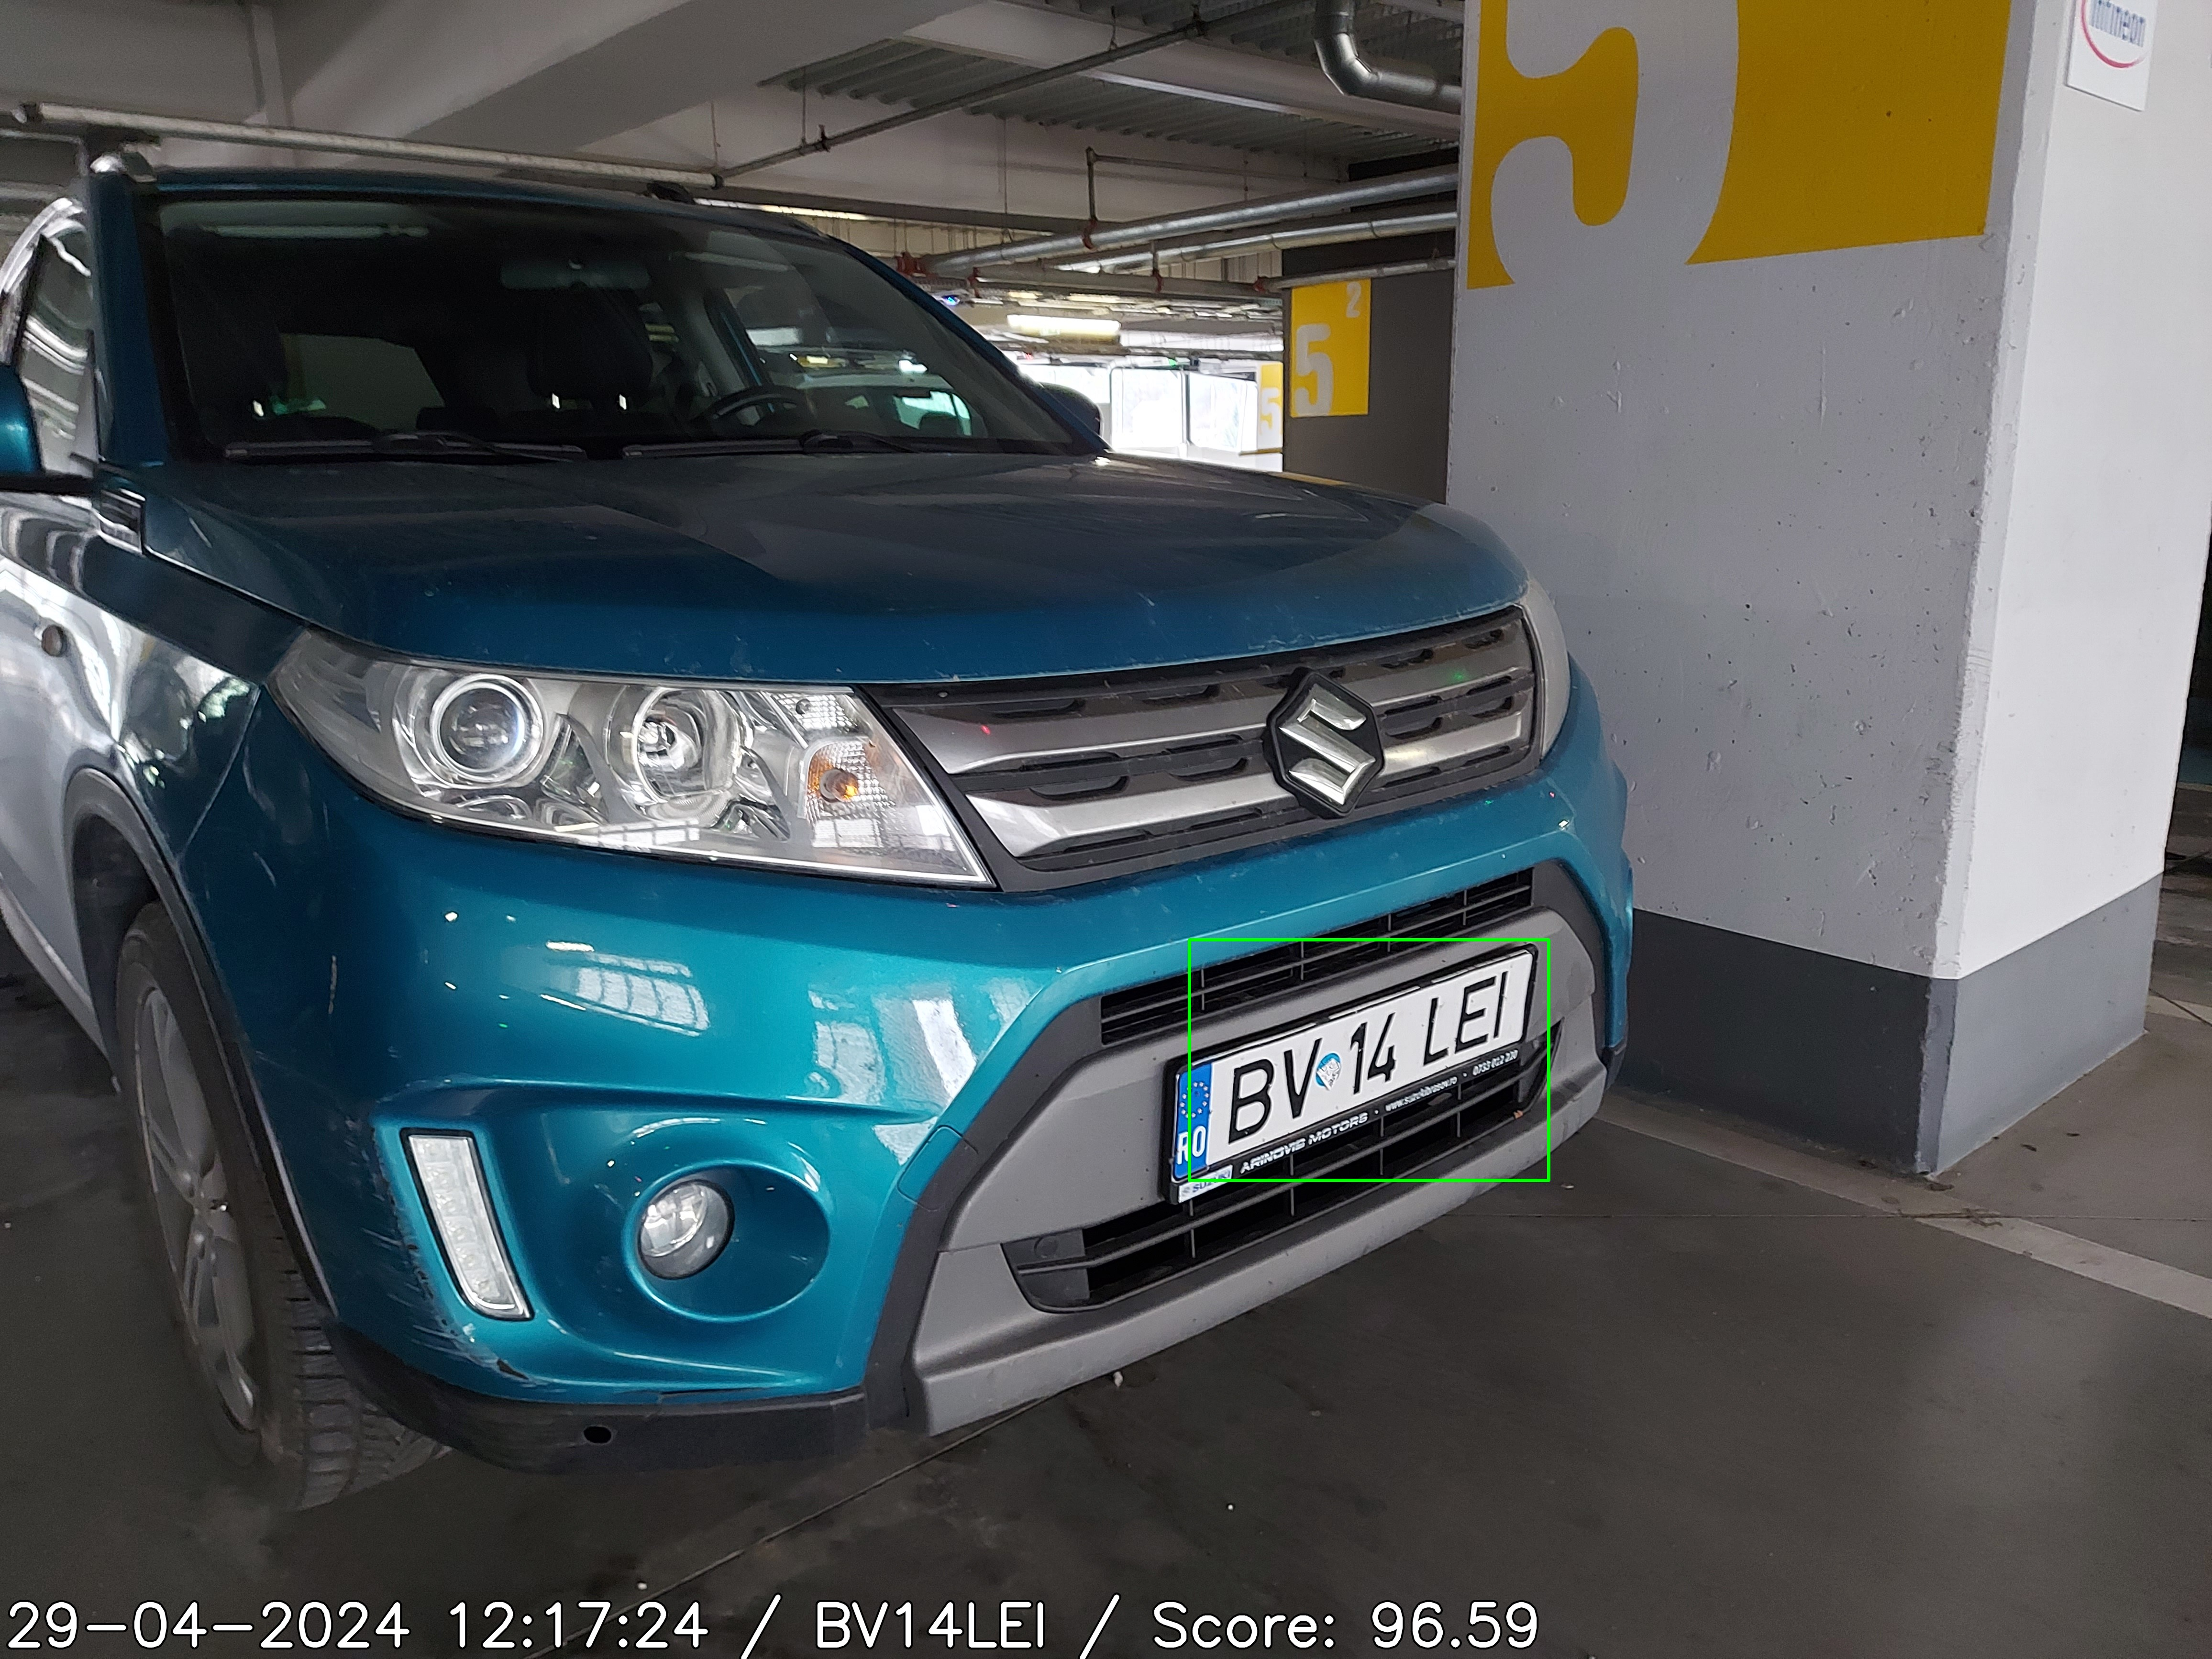
\includegraphics[width=0.4\textwidth]{images/output.jpg}
    \caption{Imaginea de output}
\end{figure}
\FloatBarrier

În situația în care nu a fost recunoscut textul integral al numărului de înmatriculare, acesta este catalogat drept "necunoscut".

\section*{Direcții și dezvoltări viitoare}
Pentru a asigura o alternativă eficientă în cazul unor erori ale sistemului principal de recunoaștere a numerelor de înmatriculare, se prevede implementarea unui sistem de backup bazat pe tickete cu coduri de bare. Această soluție va permite accesul vehiculelor în parcarea auto prin scanarea unui cod de bare generat la intrare, asigurând astfel continuitatea serviciului chiar și în condiții neprevazute a sistemului principal.

De asemenea, se dorește dezvoltarea și configurarea unui model propriu de inteligență artificială, conceput special pentru a se adapta specificului și cerințelor sistemului de monitorizare a parcărilor. Acest model AI se vrea a fi dezvoltat utilizând tehnici de învățare automată și seturi de date extinse, pentru a îmbunătăți acuratețea și eficiența recunoașterii numerelor de înmatriculare. Procesul va include etape de antrenare si testare ale modelului, cu scopul de a optimiza performanța generală a sistemului.

Aceste doua functionalitati dovedesc inovarea continuă pentru astfel de sisteme de gestionare a accesului în parcările auto și aduc un plus de securitate, facilitând o gestionare mai flexibilă și adaptată nevoilor utilizatorilor.

\section*{Concluzii}
În procesul de dezvoltare a sistemului, competențele și cunoștințele legate de tehnologiile aplicate au cunoscut îmbunătățiri, dar mai ales în mod semnificativ următoarele aspecte:

\begin{itemize}
    \item \textbf{Algoritmica specifică procesării de imagini:} S-au aprofundat tehnici care sunt esențiale pentru manipularea și analiza imaginilor
    \item \textbf{Programare în C++:} Abilitățile de programare în acest limbaj au fost extinse, îmbunătățind capacitatea de a scrie cod eficient și optimizat pentru procesarea datelor.
    \item \textbf{Utilizarea bibliotecii OpenCV:} Expertiza în folosirea acestei biblioteci esențiale pentru procesarea imaginilor a fost amplificată, facilitând implementarea de soluții eficiente.
    \item \textbf{Modelul de inteligență artificială Tesseract OCR:} Experiența cu acest model a crescut, îmbunătățind acuratețea recunoașterii textului din imagini.
    \item \textbf{Framework-ul Qt:} Cunoștințele legate de acest framework au fost extinse, dezvoltând interfețele grafice pentru utilizator.
    \item \textbf{Uneltele CMake pentru configurarea proiectelor:} Utilizarea acestora a fost rafinată, asigurând o gestionare mai eficientă și automatizată a construcției software.
    \item \textbf{Implementarea testelor automate:} Competențele în testarea automată au fost aprofundate, garantând stabilitatea și funcționalitatea fiecărei componente a sistemului.
    \item \textbf{Doxygen pentru documentația tehnică:} Aplicarea Doxygen a fost îmbunătățită, contribuind la atingerea unui standard în documentarea codului și facilitarea înțelegerii acestuia.
    \item \textbf{Mediul de integrare Visual Studio:} Experiența cu acest mediu de dezvoltare a fost consolidată, sprijinind eficiența în scrierea codului.
    \item \textbf{GitLab pentru versionarea codului:} Utilizarea GitLab a fost îmbunătățită, în special în gestionarea versiunilor de software.
\end{itemize}

Proiectul de automatizare a accesului în parcările auto a demonstrat o serie de îmbunătățiri semnificative în eficiența operațională, securitatea sporită și gestionarea optimizată a spațiilor de parcare.

Automatizarea procesului a redus considerabil necesitatea de personal pentru verificarea manuală a accesului și a accelerat fluxul de vehicule, minimizând aglomerațiile la intrări și ieșiri.

Monitorizarea constantă și înregistrarea detaliată a tuturor vehiculelor care accesează parcarea au consolidat securitatea, facilitând identificarea rapidă a vehiculelor neautorizate sau a activităților suspecte.

Prin urmărirea exactă a vehiculelor prezente, sistemul optimizează utilizarea spațiilor disponibile și sporește planificarea mai eficientă a necesarului de parcare.

De asemenea, flexibilitatea și scalabilitatea sistemului oferă posibilitatea de extindere pentru a include mai multe camere sau pentru integrarea în rețele mai mari de parcări, furnizând o soluție adaptabilă.

Prin urmare, în urma implementării soluției descrise, s-a dezvoltat un sistem eficient de recunoaștere a numerelor de înmatriculare, care nu doar că a îmbunătățit gestionarea accesului în parcările auto, dar a și consolidat semnificativ cunoștințele de programare și competențele tehnice. Această soluție integrată a demonstrat capacitatea de a procesa și analiza imagini în condiții variate, garantând o recunoaștere rapidă și precisă a numerelor de înmatriculare.

Experiența acumulată în utilizarea tehnologiilor avansate a contribuit la dezvoltarea profesională, oferind o bază solidă pentru proiectele viitoare și pentru adaptarea continuă la noutățile tehnologice.

\section*{Anexă}
\begin{longtable}{| m{0.6cm} | m{3cm} | m{3cm} | m{1.8cm} | m{1.8cm} | m{1.8cm} |}
    \hline
    Nr. & Input & Numar de \newline înmatriculare & Text \newline țintă & Text \newline prezis & Confidența \\ \hline
    \endhead
        1 & 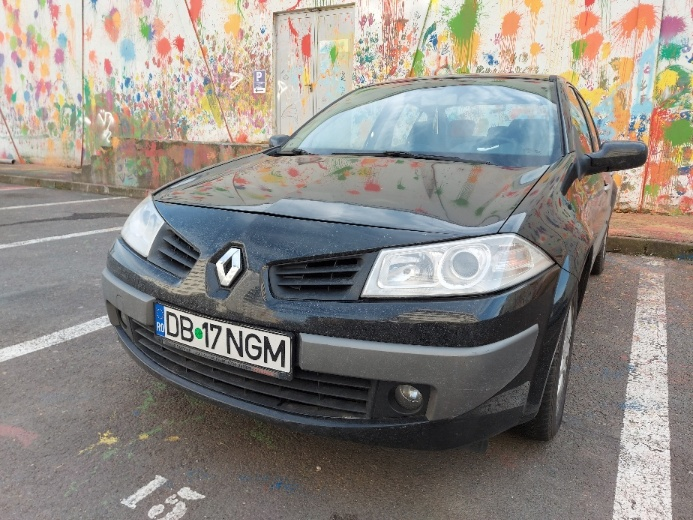
\includegraphics[width=3cm,keepaspectratio]{dataset/1_d1.jpg} & \includegraphics[width=3cm,keepaspectratio]{segmentari/1.jpg} & DB17NGM & DB17NGM & 98.97\% \\ \hline
        2 & \includegraphics[width=3cm,keepaspectratio]{dataset/1_d2.jpg} & \includegraphics[width=3cm,keepaspectratio]{segmentari/2.jpg} & DB17NGM & DB17NGM & 98.92\% \\ \hline
        3 & \includegraphics[width=3cm,keepaspectratio]{dataset/1_s1.jpg} & \includegraphics[width=3cm,keepaspectratio]{segmentari/3.jpg} & DB17NGM & DB17NGM & 98.91\% \\ \hline
        4 & \includegraphics[width=3cm,keepaspectratio]{dataset/1_s2.jpg} & \includegraphics[width=3cm,keepaspectratio]{segmentari/4.jpg} & DB17NGM & DB17NGM & 97.48\% \\ \hline
        5 & \includegraphics[width=3cm,keepaspectratio]{dataset/2_d1.jpg} & \includegraphics[width=3cm,keepaspectratio]{segmentari/5.jpg} & BV20HDY & BV20HDY & 98.74\% \\ \hline
        6 & \includegraphics[width=3cm,keepaspectratio]{dataset/2_d2.jpg} & \includegraphics[width=3cm,keepaspectratio]{segmentari/6.jpg} & BV20HDY & BV20HDY & 98.61\% \\ \hline
        7 & \includegraphics[width=3cm,keepaspectratio]{dataset/2_d3.jpg} & \includegraphics[width=3cm,keepaspectratio]{segmentari/7.jpg} & BV20HDY & BV20HDY & 98.18\% \\ \hline
        8 & \includegraphics[width=3cm,keepaspectratio]{dataset/3_d1.jpg} & \includegraphics[width=3cm,keepaspectratio]{segmentari/8.jpg} & GL87ZBM & GL87ZBM & 96.65\% \\ \hline
        9 & \includegraphics[width=3cm,keepaspectratio]{dataset/4_d1.jpg} & \includegraphics[width=3cm,keepaspectratio]{segmentari/9.jpg} & BV56RAU & BV56RAU & 97.34\% \\ \hline
        10 & \includegraphics[width=3cm,keepaspectratio]{dataset/4_d2.jpg} & \includegraphics[width=3cm,keepaspectratio]{segmentari/10.jpg} & BV56RAU & BV56RAU & 96.86\% \\ \hline
        11 & \includegraphics[width=3cm,keepaspectratio]{dataset/4_d3.jpg} & \includegraphics[width=3cm,keepaspectratio]{segmentari/11.jpg} & BV56RAU & BV56RAU & 97.37\% \\ \hline
        12 & \includegraphics[width=3cm,keepaspectratio]{dataset/5_d1.jpg} & \includegraphics[width=3cm,keepaspectratio]{segmentari/12.jpg} & BV28BRI & BV28BRI & 97.98\% \\ \hline
        13 & \includegraphics[width=3cm,keepaspectratio]{dataset/6_d1.jpg} & \includegraphics[width=3cm,keepaspectratio]{segmentari/13.jpg} & BV29PMN & BV29PMN & 98.98\% \\ \hline
        14 & \includegraphics[width=3cm,keepaspectratio]{dataset/6_d2.jpg} & \includegraphics[width=3cm,keepaspectratio]{segmentari/14.jpg} & BV29PMN & BV29PMN & 98.91\% \\ \hline
        15 & \includegraphics[width=3cm,keepaspectratio]{dataset/7_d1.jpg} & \includegraphics[width=3cm,keepaspectratio]{segmentari/15.jpg} & BV60TEO & BV60TEO & 98.38\% \\ \hline
        16 & \includegraphics[width=3cm,keepaspectratio]{dataset/7_d2.jpg} & \includegraphics[width=3cm,keepaspectratio]{segmentari/16.jpg} & BV60TEO & BV60TEO & 98.19\% \\ \hline
        17 & \includegraphics[width=3cm,keepaspectratio]{dataset/8_s1.jpg} & \includegraphics[width=3cm,keepaspectratio]{segmentari/17.jpg} & BV81NYC & BV81NYC & 97.73\% \\ \hline
        18 & \includegraphics[width=3cm,keepaspectratio]{dataset/9_d1.jpg} & \includegraphics[width=3cm,keepaspectratio]{segmentari/18.jpg} & BV20SXK & BV20SXK & 98.88\% \\ \hline
        19 & \includegraphics[width=3cm,keepaspectratio]{dataset/10_d1.jpg} & \includegraphics[width=3cm,keepaspectratio]{segmentari/19.jpg} & CT36NLA & CT36NLA & 97.66\% \\ \hline
        20 & \includegraphics[width=3cm,keepaspectratio]{dataset/10_d2.jpg} & \includegraphics[width=3cm,keepaspectratio]{segmentari/20.jpg} & CT36NLA & CT36NLA & 98.40\% \\ \hline
        21 & \includegraphics[width=3cm,keepaspectratio]{dataset/10_d3.jpg} & \includegraphics[width=3cm,keepaspectratio]{segmentari/21.jpg} & CT36NLA & CT36NLA & 98.52\% \\ \hline
        22 & \includegraphics[width=3cm,keepaspectratio]{dataset/11_d1.jpg} & \includegraphics[width=3cm,keepaspectratio]{segmentari/22.jpg} & BV18UFN & BV18UFN & 97.16\% \\ \hline
        23 & \includegraphics[width=3cm,keepaspectratio]{dataset/11_d2.jpg} & \includegraphics[width=3cm,keepaspectratio]{segmentari/23.jpg} & BV18UFN & BV18UFN & 98.20\% \\ \hline
        24 & \includegraphics[width=3cm,keepaspectratio]{dataset/12_d1.jpg} & \includegraphics[width=3cm,keepaspectratio]{segmentari/24.jpg} & BV37RED & BV37RED & 98.91\% \\ \hline
        25 & \includegraphics[width=3cm,keepaspectratio]{dataset/12_d2.jpg} & \includegraphics[width=3cm,keepaspectratio]{segmentari/25.jpg} & BV37RED & BV37RED & 98.93\% \\ \hline
        26 & \includegraphics[width=3cm,keepaspectratio]{dataset/13_d1.jpg} & \includegraphics[width=3cm,keepaspectratio]{segmentari/26.jpg} & BZ30GIG & BZ30GIG & 97.20\% \\ \hline
        27 & \includegraphics[width=3cm,keepaspectratio]{dataset/14_s1.jpg} & \includegraphics[width=3cm,keepaspectratio]{segmentari/27.jpg} & CJ25SGL & CJ25SGL & 98.44\% \\ \hline
        28 & \includegraphics[width=3cm,keepaspectratio]{dataset/15_s1.jpg} & \includegraphics[width=3cm,keepaspectratio]{segmentari/28.jpg} & AR15YCM & AR15YCM & 97.88\% \\ \hline
        29 & \includegraphics[width=3cm,keepaspectratio]{dataset/15_s2.jpg} & \includegraphics[width=3cm,keepaspectratio]{segmentari/29.jpg} & AR15YCM & AR15YCM & 97.28\% \\ \hline
        30 & \includegraphics[width=3cm,keepaspectratio]{dataset/16_s1.jpg} & \includegraphics[width=3cm,keepaspectratio]{segmentari/30.jpg} & B708VDF & B708VDF & 98.61\% \\ \hline
        31 & \includegraphics[width=3cm,keepaspectratio]{dataset/16_s2.jpg} & \includegraphics[width=3cm,keepaspectratio]{segmentari/31.jpg} & B708VDF & B708VDF & 98.63\% \\ \hline
        32 & \includegraphics[width=3cm,keepaspectratio]{dataset/17_s1.jpg} & \includegraphics[width=3cm,keepaspectratio]{segmentari/32.jpg} & BV90WLF & BV90WLF & 98.58\% \\ \hline
        33 & \includegraphics[width=3cm,keepaspectratio]{dataset/18_s1.jpg} & \includegraphics[width=3cm,keepaspectratio]{segmentari/33.jpg} & BV77RSU & BV77RSU & 98.96\% \\ \hline
        34 & \includegraphics[width=3cm,keepaspectratio]{dataset/19_d1.jpg} & \includegraphics[width=3cm,keepaspectratio]{segmentari/34.jpg} & BV02ALA & BV02ALA & 99.13\% \\ \hline
        35 & \includegraphics[width=3cm,keepaspectratio]{dataset/20_d1.jpg} & \includegraphics[width=3cm,keepaspectratio]{segmentari/35.jpg} & B730HEX & B730HEX & 98.96\% \\ \hline
        36 & \includegraphics[width=3cm,keepaspectratio]{dataset/21_d1.jpg} & \includegraphics[width=3cm,keepaspectratio]{segmentari/36.jpg} & B88FBU & B88FBU & 98.89\% \\ \hline
        37 & \includegraphics[width=3cm,keepaspectratio]{dataset/21_d2.jpg} & \includegraphics[width=3cm,keepaspectratio]{segmentari/37.jpg} & B88FBU & B88FBU & 98.82\% \\ \hline
        38 & \includegraphics[width=3cm,keepaspectratio]{dataset/21_d3.jpg} & \includegraphics[width=3cm,keepaspectratio]{segmentari/38.jpg} & B88FBU & B88FBU & 98.90\% \\ \hline
        39 & \includegraphics[width=3cm,keepaspectratio]{dataset/22_d1.jpg} & \includegraphics[width=3cm,keepaspectratio]{segmentari/39.jpg} & DB20PMD & DB20PMD & 98.67\% \\ \hline
        40 & \includegraphics[width=3cm,keepaspectratio]{dataset/23_d1.jpg} & \includegraphics[width=3cm,keepaspectratio]{segmentari/40.jpg} & B496AMI & B496AMI & 98.33\% \\ \hline
        41 & \includegraphics[width=3cm,keepaspectratio]{dataset/24_d1.jpg} & \includegraphics[width=3cm,keepaspectratio]{segmentari/41.jpg} & BV15ZTP & BV15ZTP & 97.09\% \\ \hline
        42 & \includegraphics[width=3cm,keepaspectratio]{dataset/24_s1.jpg} & \includegraphics[width=3cm,keepaspectratio]{segmentari/42.jpg} & BV15ZTP & BV15ZTP & 97.88\% \\ \hline
        43 & \includegraphics[width=3cm,keepaspectratio]{dataset/25_d1.jpg} & \includegraphics[width=3cm,keepaspectratio]{segmentari/43.jpg} & BV20ZZB & BV20ZZB & 98.21\% \\ \hline
        44 & \includegraphics[width=3cm,keepaspectratio]{dataset/25_s1.jpg} & \includegraphics[width=3cm,keepaspectratio]{segmentari/44.jpg} & BV20ZZB & BV20ZZB & 97.97\% \\ \hline
        45 & \includegraphics[width=3cm,keepaspectratio]{dataset/26_d1.jpg} & \includegraphics[width=3cm,keepaspectratio]{segmentari/45.jpg} & BV15TWB & BV15TWB & 97.69\% \\ \hline
        46 & \includegraphics[width=3cm,keepaspectratio]{dataset/26_s1.jpg} & \includegraphics[width=3cm,keepaspectratio]{segmentari/46.jpg} & BV15TWB & BV15TWB & 97.95\% \\ \hline
        47 & \includegraphics[width=3cm,keepaspectratio]{dataset/27_d1.jpg} & \includegraphics[width=3cm,keepaspectratio]{segmentari/47.jpg} & B808JDM & B808JDM & 99.12\% \\ \hline
        48 & \includegraphics[width=3cm,keepaspectratio]{dataset/27_s1.jpg} & \includegraphics[width=3cm,keepaspectratio]{segmentari/48.jpg} & B808JDM & B808JDM & 99.04\% \\ \hline
        49 & \includegraphics[width=3cm,keepaspectratio]{dataset/28_d1.jpg} & \includegraphics[width=3cm,keepaspectratio]{segmentari/49.jpg} & B800JDM & B800JDM & 98.86\% \\ \hline
        50 & \includegraphics[width=3cm,keepaspectratio]{dataset/28_s1.jpg} & \includegraphics[width=3cm,keepaspectratio]{segmentari/50.jpg} & B800JDM & B800JDM & 98.62\% \\ \hline
        51 & \includegraphics[width=3cm,keepaspectratio]{dataset/29_d1.jpg} & \includegraphics[width=3cm,keepaspectratio]{segmentari/51.jpg} & BV13KPM & BV13KPM & 97.88\% \\ \hline
        52 & \includegraphics[width=3cm,keepaspectratio]{dataset/29_d2.jpg} & \includegraphics[width=3cm,keepaspectratio]{segmentari/52.jpg} & BV13KPM & BV13KPM & 96.99\% \\ \hline
        53 & \includegraphics[width=3cm,keepaspectratio]{dataset/29_s1.jpg} & \includegraphics[width=3cm,keepaspectratio]{segmentari/53.jpg} & BV13KPM & BV13KPM & 98.45\% \\ \hline
        54 & \includegraphics[width=3cm,keepaspectratio]{dataset/30_d1.jpg} & \includegraphics[width=3cm,keepaspectratio]{segmentari/54.jpg} & BV19MDZ & BV19MDZ & 98.38\% \\ \hline
        55 & \includegraphics[width=3cm,keepaspectratio]{dataset/30_s1.jpg} & \includegraphics[width=3cm,keepaspectratio]{segmentari/55.jpg} & BV19MDZ & BV19MDZ & 97.62\% \\ \hline
        56 & \includegraphics[width=3cm,keepaspectratio]{dataset/31_d1.jpg} & \includegraphics[width=3cm,keepaspectratio]{segmentari/56.jpg} & BV88UMK & BV88UMK & 98.91\% \\ \hline
        57 & \includegraphics[width=3cm,keepaspectratio]{dataset/32_d1.jpg} & \includegraphics[width=3cm,keepaspectratio]{segmentari/57.jpg} & BV17XSA & BV17XSA & 98.82\% \\ \hline
        58 & \includegraphics[width=3cm,keepaspectratio]{dataset/32_s1.jpg} & \includegraphics[width=3cm,keepaspectratio]{segmentari/58.jpg} & BV17XSA & BV17XSA & 98.54\% \\ \hline
        59 & \includegraphics[width=3cm,keepaspectratio]{dataset/33_d1.jpg} & \includegraphics[width=3cm,keepaspectratio]{segmentari/59.jpg} & B500FMP & B500FMP & 97.63\% \\ \hline
        60 & \includegraphics[width=3cm,keepaspectratio]{dataset/34_d1.jpg} & \includegraphics[width=3cm,keepaspectratio]{segmentari/60.jpg} & VN61AVM & VN61AVM & 98.46\% \\ \hline
        61 & \includegraphics[width=3cm,keepaspectratio]{dataset/35_d1.jpg} & \includegraphics[width=3cm,keepaspectratio]{segmentari/61.jpg} & BV88BMG & BV88BMG & 98.93\% \\ \hline
        62 & \includegraphics[width=3cm,keepaspectratio]{dataset/35_s1.jpg} & \includegraphics[width=3cm,keepaspectratio]{segmentari/62.jpg} & BV88BMG & BV88BMG & 98.91\% \\ \hline
        63 & \includegraphics[width=3cm,keepaspectratio]{dataset/36_d1.jpg} & \includegraphics[width=3cm,keepaspectratio]{segmentari/63.jpg} & B110SRH & B110SRH & 98.09\% \\ \hline
        64 & \includegraphics[width=3cm,keepaspectratio]{dataset/36_s1.jpg} & \includegraphics[width=3cm,keepaspectratio]{segmentari/64.jpg} & B110SRH & B110SRH & 97.57\% \\ \hline
        65 & \includegraphics[width=3cm,keepaspectratio]{dataset/37_d1.jpg} & \includegraphics[width=3cm,keepaspectratio]{segmentari/65.jpg} & CV89COX & CV89COX & 98.83\% \\ \hline
        66 & \includegraphics[width=3cm,keepaspectratio]{dataset/37_s1.jpg} & \includegraphics[width=3cm,keepaspectratio]{segmentari/66.jpg} & CV89COX & CV89COX & 97.89\% \\ \hline
        67 & \includegraphics[width=3cm,keepaspectratio]{dataset/38_d1.jpg} & \includegraphics[width=3cm,keepaspectratio]{segmentari/67.jpg} & BV99VDV & BV99VDV & 99.01\% \\ \hline
        68 & \includegraphics[width=3cm,keepaspectratio]{dataset/38_s1.jpg} & \includegraphics[width=3cm,keepaspectratio]{segmentari/68.jpg} & BV99VDV & BV99VDV & 98.85\% \\ \hline
        69 & \includegraphics[width=3cm,keepaspectratio]{dataset/39_d1.jpg} & \includegraphics[width=3cm,keepaspectratio]{segmentari/69.jpg} & BV32GHE & BV32GHE & 98.85\% \\ \hline
        70 & \includegraphics[width=3cm,keepaspectratio]{dataset/39_s1.jpg} & \includegraphics[width=3cm,keepaspectratio]{segmentari/70.jpg} & BV32GHE & BV32GHE & 98.95\% \\ \hline
        71 & \includegraphics[width=3cm,keepaspectratio]{dataset/40_d1.jpg} & \includegraphics[width=3cm,keepaspectratio]{segmentari/71.jpg} & B212FAD & B212FAD & 99.08\% \\ \hline
        72 & \includegraphics[width=3cm,keepaspectratio]{dataset/40_s1.jpg} & \includegraphics[width=3cm,keepaspectratio]{segmentari/72.jpg} & B212FAD & B212FAD & 99.11\% \\ \hline
        73 & \includegraphics[width=3cm,keepaspectratio]{dataset/41_d1.jpg} & \includegraphics[width=3cm,keepaspectratio]{segmentari/73.jpg} & BV01UBC & BV01UBC & 98.28\% \\ \hline
        74 & \includegraphics[width=3cm,keepaspectratio]{dataset/42_d1.jpg} & \includegraphics[width=3cm,keepaspectratio]{segmentari/74.jpg} & NT11TRP & NT11TRP & 98.16\% \\ \hline
        75 & \includegraphics[width=3cm,keepaspectratio]{dataset/43_d1.jpg} & \includegraphics[width=3cm,keepaspectratio]{segmentari/75.jpg} & B321KWL & B321KWL & 99.13\% \\ \hline
        76 & \includegraphics[width=3cm,keepaspectratio]{dataset/43_d2.jpg} & \includegraphics[width=3cm,keepaspectratio]{segmentari/76.jpg} & B321KWL & B321KWL & 99.02\% \\ \hline
        77 & \includegraphics[width=3cm,keepaspectratio]{dataset/43_s1.jpg} & \includegraphics[width=3cm,keepaspectratio]{segmentari/77.jpg} & B321KWL & B321KWL & 98.42\% \\ \hline
        78 & \includegraphics[width=3cm,keepaspectratio]{dataset/44_d1.jpg} & \includegraphics[width=3cm,keepaspectratio]{segmentari/78.jpg} & BV83ALE & BV83ALE & 99.07\% \\ \hline
        79 & \includegraphics[width=3cm,keepaspectratio]{dataset/44_s1.jpg} & \includegraphics[width=3cm,keepaspectratio]{segmentari/79.jpg} & BV83ALE & BV83ALE & 98.99\% \\ \hline
        80 & \includegraphics[width=3cm,keepaspectratio]{dataset/45_s1.jpg} & \includegraphics[width=3cm,keepaspectratio]{segmentari/80.jpg} & SV10URK & SV10URK & 98.43\% \\ \hline
        81 & \includegraphics[width=3cm,keepaspectratio]{dataset/46_s1.jpg} & \includegraphics[width=3cm,keepaspectratio]{segmentari/81.jpg} & IS99GTM & IS99GTM & 98.73\% \\ \hline
        82 & \includegraphics[width=3cm,keepaspectratio]{dataset/47_s1.jpg} & \includegraphics[width=3cm,keepaspectratio]{segmentari/82.jpg} & CV09BDL & CV09BDL & 98.64\% \\ \hline
        83 & \includegraphics[width=3cm,keepaspectratio]{dataset/48_s1.jpg} & \includegraphics[width=3cm,keepaspectratio]{segmentari/83.jpg} & BV50MBA & BV50MBA & 98.50\% \\ \hline
        84 & \includegraphics[width=3cm,keepaspectratio]{dataset/49_d1.jpg} & \includegraphics[width=3cm,keepaspectratio]{segmentari/84.jpg} & BV94MTN & BV94MTN & 98.80\% \\ \hline
        85 & \includegraphics[width=3cm,keepaspectratio]{dataset/50_d1.jpg} & \includegraphics[width=3cm,keepaspectratio]{segmentari/85.jpg} & BV18GBT & BV18GBT & 98.80\% \\ \hline
        86 & \includegraphics[width=3cm,keepaspectratio]{dataset/51_d1.jpg} & \includegraphics[width=3cm,keepaspectratio]{segmentari/86.jpg} & BV26USA & BV26USA & 98.83\% \\ \hline
        87 & \includegraphics[width=3cm,keepaspectratio]{dataset/52_d1.jpg} & \includegraphics[width=3cm,keepaspectratio]{segmentari/87.jpg} & BV43BDL & BV43BDL & 98.31\% \\ \hline
        88 & \includegraphics[width=3cm,keepaspectratio]{dataset/52_s1.jpg} & \includegraphics[width=3cm,keepaspectratio]{segmentari/88.jpg} & BV43BDL & BV43BDL & 98.23\% \\ \hline
        89 & \includegraphics[width=3cm,keepaspectratio]{dataset/53_d1.jpg} & \includegraphics[width=3cm,keepaspectratio]{segmentari/89.jpg} & CV07BJM & CV07BJM & 99.04\% \\ \hline
        90 & \includegraphics[width=3cm,keepaspectratio]{dataset/53_s1.jpg} & \includegraphics[width=3cm,keepaspectratio]{segmentari/90.jpg} & CV07BJM & CV07BJM & 98.64\% \\ \hline
        91 & \includegraphics[width=3cm,keepaspectratio]{dataset/54_d1.jpg} & \includegraphics[width=3cm,keepaspectratio]{segmentari/91.jpg} & BV30PAG & BV30PAG & 98.90\% \\ \hline
        92 & \includegraphics[width=3cm,keepaspectratio]{dataset/54_s1.jpg} & \includegraphics[width=3cm,keepaspectratio]{segmentari/92.jpg} & BV30PAG & BV30PAG & 98.48\% \\ \hline
        93 & \includegraphics[width=3cm,keepaspectratio]{dataset/55_d1.jpg} & \includegraphics[width=3cm,keepaspectratio]{segmentari/93.jpg} & BV63TOY & BV63TOY & 98.15\% \\ \hline
        94 & \includegraphics[width=3cm,keepaspectratio]{dataset/55_s1.jpg} & \includegraphics[width=3cm,keepaspectratio]{segmentari/94.jpg} & BV63TOY & BV63TOY & 97.95\% \\ \hline
        95 & \includegraphics[width=3cm,keepaspectratio]{dataset/56_d1.jpg} & \includegraphics[width=3cm,keepaspectratio]{segmentari/95.jpg} & BV16EWM & BV16EWM & 98.50\% \\ \hline
        96 & \includegraphics[width=3cm,keepaspectratio]{dataset/56_s1.jpg} & \includegraphics[width=3cm,keepaspectratio]{segmentari/96.jpg} & BV16EWM & BV16EWM & 98.01\% \\ \hline
        97 & \includegraphics[width=3cm,keepaspectratio]{dataset/57_d1.jpg} & \includegraphics[width=3cm,keepaspectratio]{segmentari/97.jpg} & VN97CRU & VN97CRU & 98.91\% \\ \hline
        98 & \includegraphics[width=3cm,keepaspectratio]{dataset/57_s1.jpg} & \includegraphics[width=3cm,keepaspectratio]{segmentari/98.jpg} & VN97CRU & VN97CRU & 98.78\% \\ \hline
        99 & \includegraphics[width=3cm,keepaspectratio]{dataset/58_s1.jpg} & \includegraphics[width=3cm,keepaspectratio]{segmentari/99.jpg} & BV13LIE & BV13LIE & 97.41\% \\ \hline
        100 & \includegraphics[width=3cm,keepaspectratio]{dataset/59_d1.jpg} & \includegraphics[width=3cm,keepaspectratio]{segmentari/100.jpg} & B110NPA & B110NPA & 98.34\% \\ \hline
        101 & \includegraphics[width=3cm,keepaspectratio]{dataset/59_s1.jpg} & \includegraphics[width=3cm,keepaspectratio]{segmentari/101.jpg} & B110NPA & B110NPA & 98.66\% \\ \hline
        102 & \includegraphics[width=3cm,keepaspectratio]{dataset/60_d1.jpg} & \includegraphics[width=3cm,keepaspectratio]{segmentari/102.jpg} & BV26BBZ & BV26BBZ & 97.90\% \\ \hline
        103 & \includegraphics[width=3cm,keepaspectratio]{dataset/60_s1.jpg} & \includegraphics[width=3cm,keepaspectratio]{segmentari/103.jpg} & BV26BBZ & BV26BBZ & 97.29\% \\ \hline
        104 & \includegraphics[width=3cm,keepaspectratio]{dataset/61_d1.jpg} & \includegraphics[width=3cm,keepaspectratio]{segmentari/104.jpg} & B675GEO & B675GEO & 98.29\% \\ \hline
        105 & \includegraphics[width=3cm,keepaspectratio]{dataset/61_s1.jpg} & \includegraphics[width=3cm,keepaspectratio]{segmentari/105.jpg} & B675GEO & B675GEO & 96.96\% \\ \hline
        106 & \includegraphics[width=3cm,keepaspectratio]{dataset/62_d1.jpg} & \includegraphics[width=3cm,keepaspectratio]{segmentari/106.jpg} & BV24CAI & BV24CAI & 98.87\% \\ \hline
        107 & \includegraphics[width=3cm,keepaspectratio]{dataset/62_s1.jpg} & \includegraphics[width=3cm,keepaspectratio]{segmentari/107.jpg} & BV24CAI & BV24CAI & 96.98\% \\ \hline
        108 & \includegraphics[width=3cm,keepaspectratio]{dataset/63_d1.jpg} & \includegraphics[width=3cm,keepaspectratio]{segmentari/108.jpg} & BV17CLT & BV17CLT & 98.68\% \\ \hline
        109 & \includegraphics[width=3cm,keepaspectratio]{dataset/63_s1.jpg} & \includegraphics[width=3cm,keepaspectratio]{segmentari/109.jpg} & BV17CLT & BV17CLT & 98.80\% \\ \hline
        110 & \includegraphics[width=3cm,keepaspectratio]{dataset/64_d1.jpg} & \includegraphics[width=3cm,keepaspectratio]{segmentari/110.jpg} & BV19BRO & BV19BRO & 98.80\% \\ \hline
        111 & \includegraphics[width=3cm,keepaspectratio]{dataset/64_s1.jpg} & \includegraphics[width=3cm,keepaspectratio]{segmentari/111.jpg} & BV19BRO & BV19BRO & 98.25\% \\ \hline
        112 & \includegraphics[width=3cm,keepaspectratio]{dataset/65_d1.jpg} & \includegraphics[width=3cm,keepaspectratio]{segmentari/112.jpg} & BV97DIA & BV97DIA & 97.97\% \\ \hline
        113 & \includegraphics[width=3cm,keepaspectratio]{dataset/65_s1.jpg} & \includegraphics[width=3cm,keepaspectratio]{segmentari/113.jpg} & BV97DIA & BV97DIA & 97.11\% \\ \hline
        114 & \includegraphics[width=3cm,keepaspectratio]{dataset/66_s1.jpg} & \includegraphics[width=3cm,keepaspectratio]{segmentari/114.jpg} & BV07RGN & BV07RGN & 98.65\% \\ \hline
        115 & \includegraphics[width=3cm,keepaspectratio]{dataset/67_d1.jpg} & \includegraphics[width=3cm,keepaspectratio]{segmentari/115.jpg} & BV99RMB & BV99RMB & 98.90\% \\ \hline
        116 & \includegraphics[width=3cm,keepaspectratio]{dataset/67_s1.jpg} & \includegraphics[width=3cm,keepaspectratio]{segmentari/116.jpg} & BV99RMB & BV99RMB & 99.05\% \\ \hline
        117 & \includegraphics[width=3cm,keepaspectratio]{dataset/68_s1.jpg} & \includegraphics[width=3cm,keepaspectratio]{segmentari/117.jpg} & BV41AIG & BV41AIG & 96.82\% \\ \hline
        118 & \includegraphics[width=3cm,keepaspectratio]{dataset/69_d1.jpg} & \includegraphics[width=3cm,keepaspectratio]{segmentari/118.jpg} & BV17CCO & BV17CCO & 98.75\% \\ \hline
        119 & \includegraphics[width=3cm,keepaspectratio]{dataset/69_s1.jpg} & \includegraphics[width=3cm,keepaspectratio]{segmentari/119.jpg} & BV17CCO & BV17CCO & 98.63\% \\ \hline
        120 & \includegraphics[width=3cm,keepaspectratio]{dataset/70_s1.jpg} & \includegraphics[width=3cm,keepaspectratio]{segmentari/120.jpg} & BV17NFU & BV17NFU & 97.43\% \\ \hline
        121 & \includegraphics[width=3cm,keepaspectratio]{dataset/71_d1.jpg} & \includegraphics[width=3cm,keepaspectratio]{segmentari/121.jpg} & BV62MDL & BV62MDL & 98.06\% \\ \hline
        122 & \includegraphics[width=3cm,keepaspectratio]{dataset/72_d1.jpg} & \includegraphics[width=3cm,keepaspectratio]{segmentari/122.jpg} & B520DGY & B520DGY & 98.39\% \\ \hline
        123 & \includegraphics[width=3cm,keepaspectratio]{dataset/72_s1.jpg} & \includegraphics[width=3cm,keepaspectratio]{segmentari/123.jpg} & B520DGY & B520DGY & 98.50\% \\ \hline
        124 & \includegraphics[width=3cm,keepaspectratio]{dataset/73_d1.jpg} & \includegraphics[width=3cm,keepaspectratio]{segmentari/124.jpg} & BV92BBU & BV92BBU & 98.99\% \\ \hline
        125 & \includegraphics[width=3cm,keepaspectratio]{dataset/73_s1.jpg} & \includegraphics[width=3cm,keepaspectratio]{segmentari/125.jpg} & BV92BBU & BV92BBU & 99.02\% \\ \hline
        126 & \includegraphics[width=3cm,keepaspectratio]{dataset/74_d1.jpg} & \includegraphics[width=3cm,keepaspectratio]{segmentari/126.jpg} & VN99CZJ & VN99CZJ & 97.41\% \\ \hline
        127 & \includegraphics[width=3cm,keepaspectratio]{dataset/75_d1.jpg} & \includegraphics[width=3cm,keepaspectratio]{segmentari/127.jpg} & BV28NIM & BV28NIM & 98.64\% \\ \hline
        128 & \includegraphics[width=3cm,keepaspectratio]{dataset/75_s1.jpg} & \includegraphics[width=3cm,keepaspectratio]{segmentari/128.jpg} & BV28NIM & BV28NIM & 97.73\% \\ \hline
        129 & \includegraphics[width=3cm,keepaspectratio]{dataset/76_d1.jpg} & \includegraphics[width=3cm,keepaspectratio]{segmentari/129.jpg} & BV83ARC & BV83ARC & 99.00\% \\ \hline
        130 & \includegraphics[width=3cm,keepaspectratio]{dataset/76_s1.jpg} & \includegraphics[width=3cm,keepaspectratio]{segmentari/130.jpg} & BV83ARC & BV83ARC & 99.03\% \\ \hline
        131 & \includegraphics[width=3cm,keepaspectratio]{dataset/77_d1.jpg} & \includegraphics[width=3cm,keepaspectratio]{segmentari/131.jpg} & BV02LTV & BV02LTV & 98.62\% \\ \hline
        132 & \includegraphics[width=3cm,keepaspectratio]{dataset/78_d1.jpg} & \includegraphics[width=3cm,keepaspectratio]{segmentari/132.jpg} & BV70NOA & BV70NOA & 98.01\% \\ \hline
        133 & \includegraphics[width=3cm,keepaspectratio]{dataset/78_s1.jpg} & \includegraphics[width=3cm,keepaspectratio]{segmentari/133.jpg} & BV70NOA & BV70NOA & 98.65\% \\ \hline
        134 & \includegraphics[width=3cm,keepaspectratio]{dataset/79_d1.jpg} & \includegraphics[width=3cm,keepaspectratio]{segmentari/134.jpg} & BV14LEI & BV14LEI & 95.51\% \\ \hline
        135 & \includegraphics[width=3cm,keepaspectratio]{dataset/79_s1.jpg} & \includegraphics[width=3cm,keepaspectratio]{segmentari/135.jpg} & BV14LEI & BV14LEI & 96.56\% \\ \hline
        136 & \includegraphics[width=3cm,keepaspectratio]{dataset/80_d1.jpg} & \includegraphics[width=3cm,keepaspectratio]{segmentari/136.jpg} & BV61MTS & BV61MTS & 98.45\% \\ \hline
        137 & \includegraphics[width=3cm,keepaspectratio]{dataset/80_s1.jpg} & \includegraphics[width=3cm,keepaspectratio]{segmentari/137.jpg} & BV61MTS & BV61MTS & 98.69\% \\ \hline
        138 & \includegraphics[width=3cm,keepaspectratio]{dataset/81_d1.jpg} & \includegraphics[width=3cm,keepaspectratio]{segmentari/138.jpg} & BV77MRU & BV77MRU & 98.88\% \\ \hline
        139 & \includegraphics[width=3cm,keepaspectratio]{dataset/82_d1.jpg} & \includegraphics[width=3cm,keepaspectratio]{segmentari/139.jpg} & B77RHY & B77RHY & 99.09\% \\ \hline
        140 & \includegraphics[width=3cm,keepaspectratio]{dataset/82_d2.jpg} & \includegraphics[width=3cm,keepaspectratio]{segmentari/140.jpg} & B77RHY & B77RHY & 99.12\% \\ \hline
        141 & \includegraphics[width=3cm,keepaspectratio]{dataset/82_s1.jpg} & \includegraphics[width=3cm,keepaspectratio]{segmentari/141.jpg} & B77RHY & B77RHY & 95.17\% \\ \hline
        142 & \includegraphics[width=3cm,keepaspectratio]{dataset/83_d1.jpg} & \includegraphics[width=3cm,keepaspectratio]{segmentari/142.jpg} & AG95BFG & AG95BFG & 98.62\% \\ \hline
        143 & \includegraphics[width=3cm,keepaspectratio]{dataset/83_s1.jpg} & \includegraphics[width=3cm,keepaspectratio]{segmentari/143.jpg} & AG95BFG & AG95BFG & 97.17\% \\ \hline
        144 & \includegraphics[width=3cm,keepaspectratio]{dataset/84_d1.jpg} & \includegraphics[width=3cm,keepaspectratio]{segmentari/144.jpg} & BV70AAC & BV70AAC & 99.12\% \\ \hline
        145 & \includegraphics[width=3cm,keepaspectratio]{dataset/84_s1.jpg} & \includegraphics[width=3cm,keepaspectratio]{segmentari/145.jpg} & BV70AAC & BV70AAC & 99.02\% \\ \hline
        146 & \includegraphics[width=3cm,keepaspectratio]{dataset/85_d1.jpg} & \includegraphics[width=3cm,keepaspectratio]{segmentari/146.jpg} & BV03BYT & BV03BYT & 98.92\% \\ \hline
        147 & \includegraphics[width=3cm,keepaspectratio]{dataset/86_d1.jpg} & \includegraphics[width=3cm,keepaspectratio]{segmentari/147.jpg} & CV92NAT & CV92NAT & 99.11\% \\ \hline
        148 & \includegraphics[width=3cm,keepaspectratio]{dataset/87_d1.jpg} & \includegraphics[width=3cm,keepaspectratio]{segmentari/148.jpg} & AG93WAY & AG93WAY & 99.16\% \\ \hline
        149 & \includegraphics[width=3cm,keepaspectratio]{dataset/87_s1.jpg} & \includegraphics[width=3cm,keepaspectratio]{segmentari/149.jpg} & AG93WAY & AG93WAY & 99.16\% \\ \hline
        150 & \includegraphics[width=3cm,keepaspectratio]{dataset/88_d1.jpg} & \includegraphics[width=3cm,keepaspectratio]{segmentari/150.jpg} & BV19PDM & BV19PDM & 98.91\% \\ \hline
        151 & \includegraphics[width=3cm,keepaspectratio]{dataset/88_s1.jpg} & \includegraphics[width=3cm,keepaspectratio]{segmentari/151.jpg} & BV19PDM & BV19PDM & 98.77\% \\ \hline
        152 & \includegraphics[width=3cm,keepaspectratio]{dataset/89_s1.jpg} & \includegraphics[width=3cm,keepaspectratio]{segmentari/152.jpg} & BV12PDM & BV12PDM & 98.48\% \\ \hline
        153 & \includegraphics[width=3cm,keepaspectratio]{dataset/90_s1.jpg} & \includegraphics[width=3cm,keepaspectratio]{segmentari/153.jpg} & BV45MCR & BV45MCR & 98.73\% \\ \hline
        154 & \includegraphics[width=3cm,keepaspectratio]{dataset/91_s1.jpg} & \includegraphics[width=3cm,keepaspectratio]{segmentari/154.jpg} & CV92PRO & CV92PRO & 97.72\% \\ \hline
        155 & \includegraphics[width=3cm,keepaspectratio]{dataset/92_s1.jpg} & \includegraphics[width=3cm,keepaspectratio]{segmentari/155.jpg} & B211ABV & B211ABV & 98.80\% \\ \hline
        156 & \includegraphics[width=3cm,keepaspectratio]{dataset/93_s1.jpg} & \includegraphics[width=3cm,keepaspectratio]{segmentari/156.jpg} & IS03BMI & IS03BMI & 96.44\% \\ \hline
        157 & \includegraphics[width=3cm,keepaspectratio]{dataset/94_s1.jpg} & \includegraphics[width=3cm,keepaspectratio]{segmentari/157.jpg} & CV07BHS & CV07BHS & 98.76\% \\ \hline
        158 & \includegraphics[width=3cm,keepaspectratio]{dataset/95_s1.jpg} & \includegraphics[width=3cm,keepaspectratio]{segmentari/158.jpg} & CV05DIW & CV05DIW & 91.78\% \\ \hline
        159 & \includegraphics[width=3cm,keepaspectratio]{dataset/96_d1.jpg} & \includegraphics[width=3cm,keepaspectratio]{segmentari/159.jpg} & BV50MSL & BV50MSL & 98.14\% \\ \hline
        160 & \includegraphics[width=3cm,keepaspectratio]{dataset/97_d1.jpg} & \includegraphics[width=3cm,keepaspectratio]{segmentari/160.jpg} & BV09FVK & BV09FVK & 98.62\% \\ \hline
        161 & \includegraphics[width=3cm,keepaspectratio]{dataset/98_d1.jpg} & \includegraphics[width=3cm,keepaspectratio]{segmentari/161.jpg} & AG95NRS & AG95NRS & 97.60\% \\ \hline
        162 & \includegraphics[width=3cm,keepaspectratio]{dataset/99_d1.jpg} & \includegraphics[width=3cm,keepaspectratio]{segmentari/162.jpg} & BV77RSU & BV77RSU & 98.84\% \\ \hline
        163 & \includegraphics[width=3cm,keepaspectratio]{dataset/100_d1.jpg} & \includegraphics[width=3cm,keepaspectratio]{segmentari/163.jpg} & BV77ZZP & BV77ZZP & 98.29\% \\ \hline
        164 & \includegraphics[width=3cm,keepaspectratio]{dataset/101_d1.jpg} & \includegraphics[width=3cm,keepaspectratio]{segmentari/164.jpg} & BV17PVU & BV17PVU & 98.69\% \\ \hline
        165 & \includegraphics[width=3cm,keepaspectratio]{dataset/102_d1.jpg} & \includegraphics[width=3cm,keepaspectratio]{segmentari/165.jpg} & IF37MRY & IF37MRY & 98.26\% \\ \hline
        166 & \includegraphics[width=3cm,keepaspectratio]{dataset/103_d1.jpg} & \includegraphics[width=3cm,keepaspectratio]{segmentari/166.jpg} & BV94TRT & BV94TRT & 98.19\% \\ \hline
        167 & \includegraphics[width=3cm,keepaspectratio]{dataset/104_d1.jpg} & \includegraphics[width=3cm,keepaspectratio]{segmentari/167.jpg} & BV30PLK & BV30PLK & 98.87\% \\ \hline
        168 & \includegraphics[width=3cm,keepaspectratio]{dataset/105_d1.jpg} & \includegraphics[width=3cm,keepaspectratio]{segmentari/168.jpg} & BV07RGN & BV07RGN & 93.96\% \\ \hline
        169 & \includegraphics[width=3cm,keepaspectratio]{dataset/106_d1.jpg} & \includegraphics[width=3cm,keepaspectratio]{segmentari/169.jpg} & BC74DNS & BC74DNS & 97.35\% \\ \hline
        170 & \includegraphics[width=3cm,keepaspectratio]{dataset/106_s1.jpg} & \includegraphics[width=3cm,keepaspectratio]{segmentari/170.jpg} & BC74DNS & BC74DNS & 91.62\% \\ \hline
        171 & \includegraphics[width=3cm,keepaspectratio]{dataset/107_d1.jpg} & \includegraphics[width=3cm,keepaspectratio]{segmentari/171.jpg} & BC89BEJ & BC89BEJ & 98.99\% \\ \hline
        172 & \includegraphics[width=3cm,keepaspectratio]{dataset/107_s1.jpg} & \includegraphics[width=3cm,keepaspectratio]{segmentari/172.jpg} & BC89BEJ & BC89BEJ & 99.06\% \\ \hline
        173 & \includegraphics[width=3cm,keepaspectratio]{dataset/108_d1.jpg} & \includegraphics[width=3cm,keepaspectratio]{segmentari/173.jpg} & BC89MSW & BC89MSW & 99.04\% \\ \hline
        174 & \includegraphics[width=3cm,keepaspectratio]{dataset/108_s1.jpg} & \includegraphics[width=3cm,keepaspectratio]{segmentari/174.jpg} & BC89MSW & BC89MSW & 99.11\% \\ \hline
        175 & \includegraphics[width=3cm,keepaspectratio]{dataset/109_d1.jpg} & \includegraphics[width=3cm,keepaspectratio]{segmentari/175.jpg} & BC99CSI & BC99CSI & 98.45\% \\ \hline
        176 & \includegraphics[width=3cm,keepaspectratio]{dataset/109_s1.jpg} & \includegraphics[width=3cm,keepaspectratio]{segmentari/176.jpg} & BC99CSI & BC99CSI & 98.09\% \\ \hline
        177 & \includegraphics[width=3cm,keepaspectratio]{dataset/110_d1.jpg} & \includegraphics[width=3cm,keepaspectratio]{segmentari/177.jpg} & B154HIL & B154HIL & 97.15\% \\ \hline
        178 & \includegraphics[width=3cm,keepaspectratio]{dataset/110_s1.jpg} & \includegraphics[width=3cm,keepaspectratio]{segmentari/178.jpg} & B154HIL & B154HIL & 97.05\% \\ \hline
        179 & \includegraphics[width=3cm,keepaspectratio]{dataset/111_d1.jpg} & \includegraphics[width=3cm,keepaspectratio]{segmentari/179.jpg} & BC21GUZ & BC21GUZ & 98.39\% \\ \hline
        180 & \includegraphics[width=3cm,keepaspectratio]{dataset/111_s1.jpg} & \includegraphics[width=3cm,keepaspectratio]{segmentari/180.jpg} & BC21GUZ & BC21GUZ & 98.55\% \\ \hline
        181 & \includegraphics[width=3cm,keepaspectratio]{dataset/112_s1.jpg} & \includegraphics[width=3cm,keepaspectratio]{segmentari/181.jpg} & BC27TDI & BC27TDI & 97.97\% \\ \hline
        182 & \includegraphics[width=3cm,keepaspectratio]{dataset/113_d1.jpg} & \includegraphics[width=3cm,keepaspectratio]{segmentari/182.jpg} & BC05MKA & BC05MKA & 98.32\% \\ \hline
        183 & \includegraphics[width=3cm,keepaspectratio]{dataset/113_s1.jpg} & \includegraphics[width=3cm,keepaspectratio]{segmentari/183.jpg} & BC05MKA & BC05MKA & 97.96\% \\ \hline
        184 & \includegraphics[width=3cm,keepaspectratio]{dataset/114_d1.jpg} & \includegraphics[width=3cm,keepaspectratio]{segmentari/184.jpg} & BC61BSV & BC61BSV & 98.41\% \\ \hline
        185 & \includegraphics[width=3cm,keepaspectratio]{dataset/114_s1.jpg} & \includegraphics[width=3cm,keepaspectratio]{segmentari/185.jpg} & BC61BSV & BC61BSV & 98.54\% \\ \hline
        186 & \includegraphics[width=3cm,keepaspectratio]{dataset/115_s1.jpg} & \includegraphics[width=3cm,keepaspectratio]{segmentari/186.jpg} & BC27LYV & BC27LYV & 98.78\% \\ \hline
        187 & \includegraphics[width=3cm,keepaspectratio]{dataset/116_d1.jpg} & \includegraphics[width=3cm,keepaspectratio]{segmentari/187.jpg} & BC03VEL & BC03VEL & 98.80\% \\ \hline
        188 & \includegraphics[width=3cm,keepaspectratio]{dataset/117_d1.jpg} & \includegraphics[width=3cm,keepaspectratio]{segmentari/188.jpg} & BC77NDN & BC77NDN & 98.60\% \\ \hline
        189 & \includegraphics[width=3cm,keepaspectratio]{dataset/117_s1.jpg} & \includegraphics[width=3cm,keepaspectratio]{segmentari/189.jpg} & BC77NDN & BC77NDN & 99.13\% \\ \hline
        190 & \includegraphics[width=3cm,keepaspectratio]{dataset/118_d1.jpg} & \includegraphics[width=3cm,keepaspectratio]{segmentari/190.jpg} & BC23NIN & BC23NIN & 98.26\% \\ \hline
        191 & \includegraphics[width=3cm,keepaspectratio]{dataset/118_s1.jpg} & \includegraphics[width=3cm,keepaspectratio]{segmentari/191.jpg} & BC23NIN & BC23NIN & 97.64\% \\ \hline
        192 & \includegraphics[width=3cm,keepaspectratio]{dataset/118_s2.jpg} & \includegraphics[width=3cm,keepaspectratio]{segmentari/192.jpg} & BC23NIN & BC23NIN & 97.90\% \\ \hline
        \end{longtable}
\end{document}
